%!TEX program = xelatex
\documentclass[a4paper,11pt]{article}%A4纸,正文为小四号字,对应12pt
%\usepackage[UTF8]{ctex}

%Add by Karl_Lok
\usepackage[BoldFont,SlantFont,CJKchecksingle]{xeCJK}
\setCJKmainfont{SimSun}
\setCJKmonofont{SimSun}% 设置缺省中文字体

\usepackage{diagbox}

\usepackage{multido}
%\usepackage{underscore}
\usepackage{float}

\usepackage{algorithmic}

\usepackage{listings}



\usepackage{xcolor}
\lstset{escapechar=`,numbers=left
,extendedchars=false, escapeinside=`'
,basicstyle=\ttfamily
,backgroundcolor=\color[RGB]{245,245,244}
,keywordstyle=\bfseries\color[RGB]{130,0,0},identifierstyle=\bfseries\color[RGB]{0,0,130},numberstyle=\color[RGB]{41,41,255},commentstyle=\it\color[RGB]{130,130,130},stringstyle=\rmfamily\slshape\color[RGB]{255,0,0},showstringspaces=false,tabsize=4,texcl=true,frame=shadowbox,breaklines=true,float}

%设置引用
\usepackage[square]{natbib}
\bibliographystyle{GBT7714-2005NLang-UTF8} 

\setcitestyle{super}

%End

\usepackage{gzhubylw}
\begin{document}
\begin{titlepage}
	\centering
    \vspace*{0.5 cm}
    \includegraphics[scale = 0.5]{./img/logo_ucleuvenlimburg_rgb.png}\\[1cm]% University Logo
    %\textsc{\LARGE \naamschool}\\[2.0 cm]	% University Name
    %\textsc{\huge \naamschool}\\[2.0 cm]	% University Name
    \textsc{\Huge	 \naamschool}\\[2.0 cm]	% University Name

	%\textsc{\Large \coursecode}\\[1.5 cm]				% Course Code en
\textsc{\huge \coursecode}\\[1.5 cm]				% Course Code en
%\textsc{\Huge \coursecode}\\[1.5 cm]				% Course Code en

	%\textsc{\Large \info}\\[0.5 cm]				% Course Name
\textsc{\huge \info}\\[0.5 cm]				% Course Name
%\textsc{\Huge \info}\\[0.5 cm]				% Course Name
	% Title
	%\HRule \\[0.4cm]
\HRule \\[0.6cm]
	%\rule{\linewidth}{0.2 mm} \\[0.4 cm]
	{\huge \bfseries \thetitle}\\[0.4cm]
	%\rule{\linewidth}{0.2 mm} \\[1.5 cm]
	\HRule \\[1.5cm]


	% Author and supervisor
	\begin{minipage}{0.4\textwidth}
		\begin{flushleft} \large
			\emph{Auteur:}\\
			Filip Vanden Eynde
			\end{flushleft}
			\end{minipage}~
			\begin{minipage}{0.4\textwidth}
			\begin{flushright} \large
			\emph{Student Number:} \\
			r0363898									% Your Student Number
		\end{flushright}
	\end{minipage}\\[3 cm]  %\\[2 cm]
	%\end{minipage}
	%\vfill

	% Bottom of the page
    %{\large januari, 2016}
	
	%{\large \MONTH , \YEAR}%\\[2 cm]

	{\large \today}%\\[2 cm]

	\vfill
	
\end{titlepage}
%%%%%%%%%%%%%%

\makecover
\makeatletter
\begin{center}{ \textbf{ \LARGE{\@title}}}\end{center}
\makeatother
{\flushleft\textbf{\large 摘要}\hspace{2em}}
%!TEX program = XeLaTeX
%!TeX root =main.tex
%请在下面输入中文摘要。
Elgamal算法是一种常用于网上数字签名的算法,同时也是很多有特殊用途的数字签名的基础.Elgamal签名方案的安全性依赖于有限域上离散对数的计算是困难的这一数学难题.本文主要研究Elgamal数字签名方案和一种的基于Elgamal签名体制的代理签名,利用Microsoft visual c++编写程序,实现了基于Elgamal算法的数字签名与验证签名和代理签名与验证代理签名。\\
{\flushleft\textbf{\large 关键词}\hspace{2em}}
%!TEX program = XeLaTeX
%!TeX root =main.tex
%请在下面输入中文关键词,以逗号分隔。
Elgamal;数字签名;代理签名;\\
{\flushleft\textbf{\large ABSTRACT}\hspace{2em}}
%!TEX program = XeLaTeX
%!TeX root =main.tex
%请在下面输入英文摘要。
Elgamal digital signature is one of the valid algorithm for digital signature,and lots of special digital signatures are base on it. This thesis mainly studies the signature and proxy-signature based on Elgamal digital signature ,and achieve the signature and proxy-signature and verify the signature and proxy-signature based on Elgamal digital signature.\\
{\flushleft\textbf{\large KEY WORDS}\hspace{2em}}
%!TEX program = XeLaTeX
%!TeX root =main.tex
%请在下面输入英文关键词,以逗号分隔。
Elgamal;Digital Signature;Proxy-signature;
\newpage
\tableofcontents
\newpage
\section{前\hspace{1em}言}
\chapter*{Preface}
\setheader{Preface}

Preface\ldots

\begin{flushright}
{\makeatletter\itshape
    \@author \\
    Delft, January 2013
\makeatother}
\end{flushright}


\section{示例:一級標題}
\subsection{示例:二級標題}
緒論的主要作用是:要告訴讀者本文的研究主題、論證本研究主題的價值所在、提出作者對研究問題的主觀答案。

\par 在此處的內容主要包括:
\begin{enumerate}
	\item[] (1) 問題實際背景和問題界定(明確實用價值及對實際問題的專業術語表述);
	\item[] (2) 文獻綜述理(論價值定位);
	\item[]	(3) 尚待解決問題(參照點選擇);
	\item[] (4) 假設提出(創新點提出);
\end{enumerate}


\subsection{示例:二級標題}
\par 通俗地講就是:研究動機、問題背景,選題原因和實際工作的關係、研究的
重要性、研究目的、研究假設或待解決問題、名詞及定義以及研究範
圍和限制等。

\subsubsection{示例:三級標題}
\par  問題實際背景和問題界定:選題的途徑:
(1)從閱讀文獻著手;
(2)從觀察現象著手。問題實際背景是用事實和現象來描述研究問題所在和其重要性。問題界定是指用專業述語來表述所要研究的問題。
\clearpage

\subsubsection{示例:三級標題}
\par 文獻綜述:是描述目前的研究現狀並作簡要分析。可以反映作者研究
的功力和閱讀文獻的數量,是否找到研究問題的關鍵文獻及抓准文獻
的重點。評述是否切中要害,是否有獨到見解。忌諱採用講義式將有
關研究課題的理論和學派簡要地陳述一篇;忌諱輕率批評前人的不足
和錯誤;忌諱含糊不清,採用的觀點和內容不清楚來源。綜述所引用
的文獻應主要選自學術期刊或學術會議的文章。教科書或其他書籍只
能占小部分。報章雜誌的觀點不能作為論證的依據。
尚待研究問題和假設的提出:以“尚待研究問題”來指出目前研究的不足
之處,然後提出研究的假設。它表述論文的創新點所在。它是對實際
問題觀察思考和閱覽前人研究工作的結果,又是論文隨後論證工作的
起點和目標。主題先行即指著手寫作前先要構造好假設樹,然後收集
資料和證據去驗證假設的真偽。假設的表述應落實到變數層次,賦予
操作性的定義,形成操作假設。


\subsubsection{示例:英文引用}
$\backslash$citet\{f3\} 括号只有年份的引用方式,\citet{f3}\label{f3}

$\backslash$citep\{f1\} 括号中有作者与年份的引用方式\citep{f1}

\subsubsection{示例:中文引用}
$\backslash$citet\{p3\} 括号只有年份的引用方式,\citet{p3}\label{p1}

$\backslash$citep\{p1\} 括号中有作者与年份的引用方式\citep{p2}


\clearpage
\subsubsection{示例:引用文獻的位置與格式}
\par 本大學碩士、博士論文引用文獻均統一使用著者-出版年制,各篇文獻
的標注內容由著者姓氏與出版年構成,並置於“( )”內。倘若只標
注著者姓氏無法識別該人名時,可標注著者姓名。多次引用同一著者
的同一文獻,在正文中標注著者與出版年,並在“( )”外以角標的
形式著錄引文頁碼,例如:(作者,年份)
頁碼 。在正文中引用同一著者
在同一年出版的多篇文獻時,出版年後應用小寫字母 a,b,c,…區別。
在正文中引用多著者文獻時,對歐美著者只需標注第一個著者的姓,
其後附“et al”;中國著者應標注第一著者的姓名,其後附“等”字,姓
氏與“等”之間留半字元空隙。

第二次引用時右上角標注上頁 \citet{f3}$^{\pageref{f3}}$

\chapter{Background}\label{ch:background}

\begin{remark}{Outline}
In this chapter, we introduce supervised learning and fundamental concepts on
which this work builds upon. In Section~\ref{sec:2:learning-from-data}, we
first describe classification and regression learning tasks and then formally
define the notion of model. In Section~\ref{sec:2:performance-evaluation}, we
proceed with a discussion on performance evaluation and then describe, in
Section~\ref{sec:2:model-selection}, procedures for selecting the best possible
model. Finally, we conclude in Section~\ref{sec:2:classes-of-algorithms} with a
brief overview of some of the main methods in supervised learning.
\end{remark}

\section{Learning from data}
\label{sec:2:learning-from-data}

In the examples introduced in Chapter~\ref{ch:introduction}, the objective
which is sought is to find a systematic way of predicting a phenomenon given a
set of measurements. In machine learning terms, this goal is formulated as the
{\it supervised learning} task of inferring from collected data a model that
predicts the value of an output variable based on the observed values of input
variables. As such, finding an appropriate model is based on the assumption
that the output variable does not take its value at random and that there
exists a relation between the inputs and the output. In medicine for instance,
the goal is to find a decision rule (i.e., a model) from a set of past cases
(i.e., the collected data) for predicting the condition of an incoming patient
(i.e., the output value) given a set of measurements such as age, sex, blood
pressure or history (i.e., the input values).

To give a more precise formulation, let us assume as set of \textit{cases} or
\textit{objects} taken from a universe $\Omega$\label{ntn:omega}. Let us arrange the set of
measurements on a case in a pre-assigned order, i.e., take the input values to
be $x_1, x_2, ..., x_p$, where $x_j \in {\cal X}_j$\label{ntn:value-x_j}\label{ntn:space-X_j} (for $j = 1, ..., p$\label{ntn:p})
corresponds to the value of the input variable $X_j$\label{ntn:var-X_j}. Together, the input
values $(x_1, x_2, ..., x_p)$ form a $p$-dimensional input vector $\mathbf{x}$\label{ntn:sample-x}
taking its values in ${\cal X}_1 \times ... \times {\cal X}_p = {\cal X}$\label{ntn:space-X},
where ${\cal X}$ is defined as the input space. Similarly, let us define as $y
\in {\cal Y}$\label{ntn:value-y} the value of the output variable $Y$\label{ntn:var-Y}, where ${\cal Y}$\label{ntn:space-Y} is defined
as the output space\footnote{Unless stated otherwise, supervised learning is
reduced to the prediction of a \textit{single} output variable. More generally
however, this framework can be defined as the prediction of one or several
output variables.}. By definition, both the input and the output spaces are
assumed to respectively contain all possible input vectors and all possible
output values. Note that input variables are sometimes known as {\it features},
input vectors as {\it instances} or {\it samples} and the output variable as
{\it target}.

Among variables that define the problem, we distinguish between two general
types. The former correspond to quantitative variables whose values are integer
or real numbers, such as age or blood pressure. The latter correspond to
qualitative variables whose values are symbolic, such as gender or condition.
Formally, we define them as follows:

\begin{definition}
A variable $X_j$\label{ntn:var-X_j2} is \emph{ordered} if ${\cal X}_j$ is a
totally ordered set. In particular, $X_j$ is said to be \emph{numerical} if
${\cal X}_j = \mathbb{R}$.
\end{definition}

\begin{definition}
A variable $X_j$ is \emph{categorical} if ${\cal X}_j$ is a finite set of values,
without any natural order.
\end{definition}

In a typical supervised learning task, past observations are summarized by a
dataset called {\it learning set}. It consists in a set of observed input
vectors together with their actual output value and formally defined as
follows:

\begin{definition}
A \emph{learning set} ${\cal L}$\label{ntn:learning-set} is a set of $N$\label{ntn:N}
pairs of input vectors and output values $(\mathbf{x}_1, y_1), ...,
(\mathbf{x}_N, y_N)$, where $\mathbf{x}_i \in {\cal X}$ and $y_i \in {\cal Y}$.
\end{definition}

Equivalently, a set of $p$-input vectors $\mathbf{x}_i$\label{ntn:sample-x_i}
(for $i=1, ..., N$) can be denoted by a $N\times p$ matrix
$\mathbf{X}$\label{ntn:matrix-X}, whose rows $i=1, ..., N$ correspond to input
vectors $\mathbf{x}_i$ and columns $j=1, ..., p$ to input variables $X_j$.
Similarly, the corresponding output values can be written as a vector
$\mathbf{y}=(y_1, ..., y_N)$\label{ntn:vector-y}.

\begin{remark}{Data representation}
For optimal implementations of machine learning algorithms, data needs to be
represented using structures which allow for high-performance numerical
computation. In this work, code snippets are described under  the assumption
that data is represented using a data structure similar to a NumPy
array~\citep{vanderwalt:2011}.

A NumPy array is basically a multidimensional uniform collection of values, all
of the same type and organized in a given shape. For instance, a matrix
$\mathbf{X}$ can be represented as a 2-dimensional NumPy array of shape $N
\times p$ that contains numbers (e.g., floating point values or integers). This
structure allows for random access in constant time, vectorized high-level
operations and efficient memory usage.

Additionally, using a data representation which is close to the matrix
formulation, like NumPy arrays, makes it possible to write implementations that
are close to their original textbook formulation, thereby making them easier to code,
understand and maintain. \end{remark}

In this framework, the supervised learning task can be stated as learning a
function $\varphi: {\cal X} \mapsto {\cal Y}$\label{ntn:varphi} from a learning
set ${\cal L}=(\mathbf{X}, \mathbf{y})$. The objective is to find a model such
that its predictions $\varphi(\mathbf{x})$\label{ntn:varphi-x}, also denoted by
the variable $\hat{Y}$, are as good as possible. If $Y$ is a categorical
variable then the learning task is a classification problem. If $Y$ is
numerical variable, then learning task is a regression problem. Without loss of
generality, the resulting models can be defined as follows:

\begin{definition}
A \emph{classifier} or \emph{classification rule} is a function $\varphi: {\cal X}
\mapsto {\cal Y}$, where ${\cal Y}$ is a finite set of classes (or labels) denoted $\{c_1, c_2, ..., c_J\}$\label{ntn:J}\label{ntn:c_k}.
\end{definition}

\begin{definition}
A \emph{regressor} is a function $\varphi: {\cal X} \mapsto {\cal Y}$, where ${\cal Y}=\mathbb{R}$.
\end{definition}

\begin{remark}{Estimator interface}
We follow in this work the API conventions proposed by~\citet{buitinck:2013}.
Learning algorithms are described as \textit{estimator} objects implementing the
following interface:

\begin{itemize}
\item Hyper-parameters of an algorithm are all passed to the constructor of the
estimator. The constructor does not see any actual data. All it does
is to attach hyper-parameters values as public attributes to the estimator object.
\item Learning is performed in a \texttt{fit} method. This method is called with
a learning set (e.g., supplied as two arrays \texttt{X\_train} and \texttt{y\_train}). Its
task is to run a learning algorithm and to determine model-specific parameters
from the data. The \texttt{fit} method always returns the estimator object
it was called on, which now serves as a model and can be used to make predictions.
\item Predictions are performed through a \texttt{predict} method, taking
as input an array \texttt{X\_test} and producing as output the predictions for
\texttt{X\_test} based on the learned parameters. In the case of classification,
this method returns labels from ${\cal Y} = \{c_1, c_2, ..., c_J\}$. In the case of regression,
it returns numerical values from ${\cal Y} = \mathbb{R}$.
\end{itemize}

With this API, a typical supervised learning task is performed as follows:

\vskip0.3cm
\begin{pythoncode}
# Instantiate and set hyper-parameters
clf = DecisionTreeClassifier(max_depth=5)
# Learn a model from data
clf.fit(X_train, y_train)
# Make predictions on new data
y_pred = clf.predict(X_test)
\end{pythoncode}
\end{remark}


\section{Performance evaluation}
\label{sec:2:performance-evaluation}

In the statistical sense, input and output variables $X_1, ..., X_p$ and $Y$
are \textit{random variables} taking jointly their values from ${\cal X} \times
{\cal Y}$ with respect to the joint probability distribution $P(X, Y)$\label{ntn:P_XY}, where
$X$\label{ntn:vector-X} denotes the random vector $(X_1, ..., X_p)$. That is, $P(X=\mathbf{x},
Y=y)$ is the probability that random variables $X$ and $Y$ take values
$\mathbf{x}$ and $y$ from ${\cal X}$ and ${\cal Y}$ when drawing an object
uniformly at random from the universe $\Omega$.

Accordingly, using an algorithm ${\cal A}$\label{ntn:A} for learning a model\footnote{Unless
it is clear from the context, models are now denoted $\varphi_{\cal L}$\label{ntn:varphi-L} to
emphasize that they are built from the learning set ${\cal L}$.} $\varphi_{\cal
L}$ whose predictions are as good as possible can be stated as finding a model
which minimizes its expected prediction error, defined as follows:

\begin{definition}
The \emph{expected prediction error}, also known as \emph{generalization
error} or \emph{test error}, of the model $\varphi_{\cal L}$ is\footnote{$\mathbb{E}_X \{f(X)\}$ denotes the expected value of $f(x)$
(for $x \in {\cal X}$) with respect to the probability distribution of the
random variable $X$. It is defined as $$\mathbb{E}_X \{f(X)\} = \sum_{x \in {\cal
X}} P(X=x) f(x).$$}
\begin{equation}\label{eqn:generalization-error}
Err(\varphi_{\cal L}) = \mathbb{E}_{X, Y}\{ L(Y, \varphi_{\cal L}(X)) \},
\end{equation}
where ${\cal L}$ is the learning set used to build $\varphi_{\cal L}$ and $L$\label{ntn:L} is a loss
function measuring the discrepancy between its two
arguments~\citep{geurts:2002}.
\end{definition}

Equation~\ref{eqn:generalization-error} basically measures the prediction error
of $\varphi_{\cal L}$ over all possible objects in $\Omega$ (each represented by a couple
$(\mathbf{x}, y)\in {\cal X}\times{\cal Y}$), including the observed couples
from the learning set ${\cal L}$ but also all the \textit{unseen} ones from
${\cal X}\times{\cal Y} \setminus {\cal L}$. Indeed, the goal is not in fact to
make the very-most accurate predictions over the subset ${\cal L}$ of known
data, but rather to learn a model which is correct and reliable on all possible
data.

For classification, the most common loss function is the \textit{zero-one} loss
function\footnote{$1(\text{\textit{condition}})$ denotes the unit function. It
is defined as
$$1(\text{\textit{condition}}) =
\begin{cases}
1 & \text{if \textit{condition} is true}\\
0 & \text{if \textit{condition} is false}
\end{cases}.
$$} $L(Y, \varphi_{\cal L}(X)) = 1(Y \neq \varphi_{\cal L}(X))$, where all
misclassifications are equally penalized. In this case, the generalization
error of $\varphi_{\cal L}$ becomes the probability of misclassification of the model:
\begin{equation}
Err(\varphi_{\cal L}) = \mathbb{E}_{X, Y}\{ 1(Y \neq \varphi_{\cal L}(X)) \} = P(Y \neq \varphi_{\cal L}(X))
\end{equation}

Similarly, for regression, the most used loss function is the \textit{squared
error} loss $L(Y, \varphi_{\cal L}(X)) = (Y - \varphi_{\cal L}(X))^2$, where large differences
between the true values and the predicted values are penalized more heavily
than small ones. With this loss, the generalization error of the model becomes:
\begin{equation}
Err(\varphi_{\cal L}) = \mathbb{E}_{X, Y}\{ (Y - \varphi_{\cal L}(X))^2  \}
\end{equation}

\subsection{Estimating $Err(\varphi_{\cal L})$}
\label{sec:2:estimating-generalization-error}

In practice, the probability distribution $P(X, Y)$ is usually unknown, making
the direct evaluation of $Err(\varphi_{\cal L})$ infeasible. Equivalently, it
is often not possible to draw additional data, thereby making infeasible the
empirical estimation of $Err(\varphi_{\cal L})$ on a (virtually infinite) set
${\cal L}'$ drawn independently from ${\cal L}$. In most problems, ${\cal L}$
constitutes the only data available, on which both the model needs to be
learned and its generalization error estimated. As reviewed and described on
multiple occasions by several
authors~\citep{toussaint:1974,stone:1978,breiman:1984,kohavi:1995,nadeau:2003,hastie:2005,arlot:2010},
the generalization error in Equation~\ref{eqn:generalization-error} can however
be estimated in several ways.

To make notations clearer, let us first define $\overline{E}(\varphi_{\cal L}, {\cal
L}^\prime)$\label{ntn:E_bar} as the average prediction error of the model $\varphi_{\cal L}$ over the set
${\cal L}^\prime$ (possibly different from the learning set ${\cal L}$ used to produce
$\varphi_{\cal L}$), that is:
\begin{equation}
\overline{E}(\varphi_{\cal L}, {\cal L}^\prime) = \frac{1}{N^\prime} \sum_{(\mathbf{x_i}, y_i) \in {\cal L}^\prime} L(y_i, \varphi_{\cal L}(\mathbf{x_i}))
\end{equation}
where $N^\prime$ is the size of the set ${\cal L}^\prime$.

The first and simplest estimate of the generalization error is the
\textit{resubstitution estimate} or \textit{training sample estimate}. It
consists in empirically estimating $Err(\varphi_{\cal L})$ on the same data as
the learning set ${\cal L}$ used to build $\varphi_{\cal L}$, that is:
\begin{equation}\label{eqn:training-error}
\widehat{Err}^\text{train}(\varphi_{\cal L}) = \overline{E}(\varphi_{\cal L}, {\cal L})
\end{equation}
In general, the resubstitution error is a poor estimate of $Err(\varphi_{\cal L})$.
In particular, since most machine learning algorithms aim at
precisely minimizing Equation~\ref{eqn:training-error} (either directly or
indirectly), it typically results in an overly optimistic estimate of the
generalization error, which accounts for all couples $(\mathbf{x}, y)$, i.e.,
not only those from ${\cal L}$.

The second approach is the \textit{test sample estimate}. It consists in
dividing the learning set ${\cal L}$ into two disjoint sets ${\cal
L}_\text{train}$ and ${\cal L}_\text{test}$, called \textit{training set} and
\textit{test set}, and then to use each part respectively for learning a model
and estimating its generalization error. The test sample estimate of the
generalization error of the model $\varphi_{\cal L}$ that would be obtained from ${\cal
L}$ is then given as the average prediction error over ${\cal L}_\text{test}$
of the model $\varphi_{{\cal L}_\text{train}}$ built on ${\cal L}_\text{train}$:
\begin{equation}\label{eqn:test-error}
\widehat{Err}^\text{test}(\varphi_{\cal L}) = \overline{E}(\varphi_{{\cal L}_\text{train}}, {\cal L}_\text{test})
\end{equation}
As a rule-of-thumb,
${\cal L}_\text{train}$ is usually taken as $70\%$ of the samples in
${\cal L}$ and ${\cal L}_\text{test}$ as the remaining $30\%$, though
theoretical work~\citep{guyon:1997} suggests to progressively reduce the size of test set as
the size of ${\cal L}$ increases. In any case, care must be taken when splitting ${\cal
L}$ into two subsets, so that samples from ${\cal L}_\text{train}$ can be
considered independent from those in ${\cal L}_\text{test}$ and drawn from the
same distribution. This is however usually guaranteed by drawing ${\cal
L}_\text{train}$ and ${\cal L}_\text{test}$ simply at random from ${\cal L}$.
While being an unbiased estimate of $Err(\varphi_{\cal L})$, the test sample
estimate has the drawback that it reduces the
effective sample size on which the model $\varphi_{{\cal L}_\text{train}}$ is learned. If ${\cal L}$ is large,
then this is usually not an issue, but if ${\cal L}$ only contains a few dozens
of samples, then this strategy might not correctly approximate the true
generalization error of the model that would have been learned on the entire learning set.

When ${\cal L}$ is small, the \textit{$K$-fold cross-validation estimate}\label{ntn:K-cv} is
usually preferred over the test sample estimate. It consists in randomly
dividing the learning set ${\cal L}$ into $K$ disjoint subsets, ${\cal
L}_1, ..., {\cal L}_K$\label{ntn:L_k}, and then to estimate the generalization error as the average prediction error over the folds ${\cal
L}_k$ of the models $\varphi_{{\cal L}\setminus {\cal L}_k}$  learned on the
remaining data:
\begin{equation}\label{eqn:cv-error}
\widehat{Err}^{CV}(\varphi_{\cal L}) = \frac{1}{K} \sum_{k=1}^K  \overline{E}(\varphi_{{\cal L}\setminus{\cal L}_k}, {\cal L}_k)
\end{equation}
The assumption behind this approach is that since each model $\varphi_{{\cal L}\setminus{\cal L}_k}$ is
built using almost all ${\cal L}$, they should all be close to the model
$\varphi_{\cal L}$ learned on the entire set. As a result the unbiased
estimates $\overline{E}(\varphi_{{\cal L}\setminus{\cal L}_k}, {\cal L}_k)$ should also all be close to
$Err(\varphi_{\cal L})$. While more computationally intensive, the $K$-fold
cross-validation estimate has the advantage that every couple $(\mathbf{x}, y)
\in {\cal L}$ is used for estimating the generalization error of $\varphi_{\cal L}$. In
a typical setting, $K$ is usually fixed to $10$, a value often yielding stable
and reliable estimates~\citep{kohavi:1995}.

\begin{remark}{Expected generalization error}
As we have shown, our goal is to estimate the generalization error
$Err(\varphi_{\cal L})$ conditional on the learning set ${\cal L}$. A related
quantity is the \textit{expected} generalization error
\begin{equation}\label{eqn:expected-generalization-error}
\mathbb{E}_{\cal L} \{ Err(\varphi_{\cal L}) \},
\end{equation}
averaging over everything which is random, including the randomness in the
learning set ${\cal L}$ used to produce $\varphi_{\cal L}$. As discussed by
\citet{hastie:2005}, this quantity is close, yet different from
$Err(\varphi_{\cal L})$. The authors point out that most estimates, including $K$-fold
cross-validation, effectively estimate
Equation~\ref{eqn:expected-generalization-error} rather than
Equation~\ref{eqn:generalization-error}.
\end{remark}

\subsection{Bayes model and residual error}
\label{sec:2:bayes-model}

In theory, when the probability distribution $P(X, Y)$ is known, the best possible model,
i.e., the model $\varphi_B$ which minimizes the generalization error of
Equation~\ref{eqn:generalization-error}, can be derived analytically and
independently of any learning set ${\cal L}$.
By conditioning on $X$, the generalization error of this model can be rewritten as:
\begin{equation}\label{eqn:generalization-error-conditionned}
\mathbb{E}_{X, Y}\{ L(Y, \varphi_B(X)) \} = \mathbb{E}_{X}\{ \mathbb{E}_{Y|X} \{ L(Y, \varphi_B(X)) \} \}
\end{equation}
In this latter form, the model which minimizes
Equation~\ref{eqn:generalization-error-conditionned} is a model which
minimizes the inner expectation point-wise, that is:
\begin{equation}
\varphi_B(\mathbf{x}) = \argmin_{y \in {\cal Y}} \mathbb{E}_{Y|X=\mathbf{x}} \{ L(Y, y) \}
\end{equation}
In the literature, $\varphi_B$ is known as the \textit{Bayes model} and its
generalization error $Err(\varphi_B)$ as the \textit{residual error}. It represents the minimal
error that any supervised learning algorithm can possibly attain, that is
the irreducible error purely due to random deviations in the data.

\begin{definition}
A model $\varphi_B$\label{ntn:varphi-B} is a \emph{Bayes model} if, for any model $\varphi$ built from any
learning set ${\cal L}$, $Err(\varphi_B) \leq Err(\varphi_{\cal L})$.
\end{definition}

In classification, when $L$ is the zero-one loss, the Bayes model is:
\begin{align}
\varphi_B(\mathbf{x}) &= \argmin_{y \in {\cal Y}} \mathbb{E}_{Y|X=\mathbf{x}} \{ 1(Y, y) \} \nonumber \\
                      &= \argmin_{y \in {\cal Y}} P(Y \neq y|X=\mathbf{x}) \nonumber \\
                      &= \argmax_{y \in {\cal Y}} P(Y = y|X=\mathbf{x}) \label{eqn:bayes-model-classification}
\end{align}
Put otherwise, the best possible classifier
consists in systematically predicting the most likely class $y \in \{c_1, c_2, ..., c_J\}$
given $X=\mathbf{x}$.

Similarly, for regression with the squared error loss, we have:
\begin{align}
\varphi_B(\mathbf{x}) &= \argmin_{y \in {\cal Y}} \mathbb{E}_{Y|X=\mathbf{x}} \{ (Y - y)^2 \} \nonumber \\
                      &= \mathbb{E}_{Y|X=\mathbf{x}} \{ Y \} \label{eqn:bayes-model-regression}
\end{align}
In other words, the best possible regressor consists in systematically predicting
the average value of $Y$ at $X=\mathbf{x}$.

For practical problems, $P(X, Y)$ is unknown and the Bayes model cannot be
derived analytically. In this context, the effectiveness of a model $\varphi_{\cal L}$
may be difficult to evaluate since (estimates of) $Err(\varphi_{\cal L})$ may
not be very indicative of the goodness of $\varphi_{\cal L}$ if the lowest attainable
error $Err(\varphi_B)$ is unknown. On simulated data however, where the
distribution is known, deriving $\varphi_B$ and $Err(\varphi_B)$ is feasible.
This is beneficial as $Err(\varphi_B)$ can now be used for comparing the test
set error of $\varphi_{\cal L}$ and thereby evaluate the actual effectiveness of
$\varphi_{\cal L}$ with respect to the best model one can possibly build.

From a theoretical point of view, the concepts of Bayes model and residual
error are also useful to study the learning capabilities of an algorithm. In
particular, as ${\cal L}$ gets arbitrarily large, a fundamental question is to
know whether it is possible to produce a model $\varphi_{\cal L}$ which is
\textit{consistent}, that is such that its generalization error gets
arbitrarily close to the lowest possible generalization error $Err(\varphi_B)$.
Formally, consistency is defined as follows~\citep{devroye:1996}:

\begin{definition}\label{def:consistency}
A learning algorithm ${\cal A}$ is said to be \emph{weakly consistent} for a certain distribution
$P(X, Y)$ if $\mathbb{E}_{\cal L} \{ Err(\varphi_{\cal L}) \} \to Err(\varphi_B)$
as the size $N$ of the learning set ${\cal L}$ used to build $\varphi_{\cal L}$ using ${\cal A}$ tends
to infinity.
\end{definition}

\begin{definition}\label{def:consistency-strong}
A learning algorithm ${\cal A}$ is said to be \emph{strongly consistent} for a certain distribution
$P(X, Y)$ if $Err(\varphi_{\cal L}) \to Err(\varphi_B)$ almost surely
as the size $N$ of the learning set ${\cal L}$ used to build $\varphi_{\cal L}$ using ${\cal A}$ tends
to infinity.
\end{definition}

Note that the definition of consistency depends on the distribution $P(X, Y)$.
In general, a learning algorithm ${\cal A}$ can be proven to be consistent for some
classes of distributions, but not for others. If consistency can be proven
for any distribution $P(X, Y)$, then ${\cal A}$ is said to be \textit{universally}
(strongly) consistent.


\section{Model selection}
\label{sec:2:model-selection}

From the previous discussion in Section~\ref{sec:2:bayes-model}, it appears that
to solve the supervised learning problem it would be sufficient to estimate
$P(Y|X)$ from the learning sample ${\cal L}$ and then to define a model
accordingly using either Equation~\ref{eqn:bayes-model-classification} or
Equation~\ref{eqn:bayes-model-regression}. Unfortunately, this approach is
infeasible in practice because it requires ${\cal L}$ to grow exponentially
with the number $p$ of input variables in order to compute accurate estimates of
$P(Y|X)$~\citep{geurts:2002}.

\subsection{Selecting the (approximately) best model}

To make supervised learning work in high-dimensional input spaces with learning
sets of moderate sizes, simplifying assumptions must be made on
the structure of the best model $\varphi_B$. More specifically, a supervised
learning algorithm assumes that $\varphi_B$ -- or at least a good enough approximation
-- lives in a family ${\cal H}$\label{ntn:H} of candidate models, also known as
\textit{hypotheses} in statistical learning theory, of restricted structure. In
this setting, the \textit{model selection} problem is then defined as finding
the best model among ${\cal H}$ on the basis of the learning set ${\cal L}$.

\begin{remark}{Approximation error}
Depending on restrictions made on the structure of the problem, the
Bayes model usually does not belong to ${\cal H}$, but there may be models
$\varphi \in {\cal H}$ that are sufficiently close to it. As such, the
\textit{approximation error}~\citep{bottou:2011} measures how closely the
models in ${\cal H}$ can approximate the optimal model $\varphi_B$:
\begin{equation}
Err({\cal H}) = \min_{\varphi \in {\cal H}} \{ Err(\varphi) \} - Err(\varphi_B)
\end{equation}
\end{remark}

To be more specific, let $\theta$\label{ntn:theta} be the vector of hyper-parameters values
controlling the execution of a learning algorithm ${\cal A}$. The application
of ${\cal A}$ with hyper-parameters $\theta$ on the learning set ${\cal L}$ is a
deterministic\footnote{If ${\cal A}$ makes use of a pseudo-random generator to
mimic a stochastic process, then we assume that the corresponding random seed is
part of $\theta$.} process yielding a model ${\cal A}(\theta, {\cal L}) =
\varphi_{\cal L} \in {\cal H}$\label{ntn:A-func}. As such, our goal is to find the vector of hyper-parameters values
yielding to the best model possibly learnable in ${\cal H}$ from ${\cal L}$:
\begin{equation}
\theta^* = \argmin_{\theta} Err({\cal A}(\theta, {\cal L}))
\end{equation}\label{ntn:theta-star}
Again, this problem cannot (usually) be solved exactly in practice since
it requires the true generalization error of a model to be computable. However
approximations $\widehat{\theta}^*$\label{ntn:theta-star-approx} can be obtained in several ways.

When ${\cal L}$ is large, the easiest way to find $\widehat{\theta}^*$ is to
use test sample estimates (as defined by Equation~\ref{eqn:test-error}) to
guide the search of the hyper-parameter values, that is:
\begin{align}
\widehat{\theta}^* &= \argmin_{\theta} \widehat{Err}^\text{test}({\cal A}(\theta, {\cal L})) \\
                   &= \argmin_{\theta} \overline{E}({\cal A}(\theta, {\cal L}_\text{train}), {\cal L}_\text{test})
\end{align}
In practice, solving this later equation is also a difficult task but
approximations can be obtained in several ways, e.g., using either manual
tuning of $\theta$, exhaustive exploration of the parameter space using grid
search, or dedicated optimization procedures (e.g., using random
search~\citep{bergstra:2012}). Similarly, when ${\cal L}$ is scarce, the same
procedure can be carried out in the exact same way but using $K$-fold
cross-validation estimates (as defined by Equation~\ref{eqn:cv-error}) instead of test sample
estimates. In any case, once $\widehat{\theta}^*$ is identified, the learning
algorithm is run once again on the entire learning set ${\cal L}$, finally
yielding the approximately optimal model ${\cal A}(\widehat{\theta}^*, {\cal
L})$.

When optimizing $\theta$, special care must be taken so that the resulting model
is neither too simple nor too complex. In the former case, the model is indeed
said to \textit{underfit} the data, i.e., to be not flexible enough the capture
the structure between $X$ and $Y$. In the later case, the model is said to
\textit{overfit} the data, i.e., to be too flexible and to capture isolated
structures (i.e., noise) that are specific to the learning set.

\begin{figure}
    \centering
    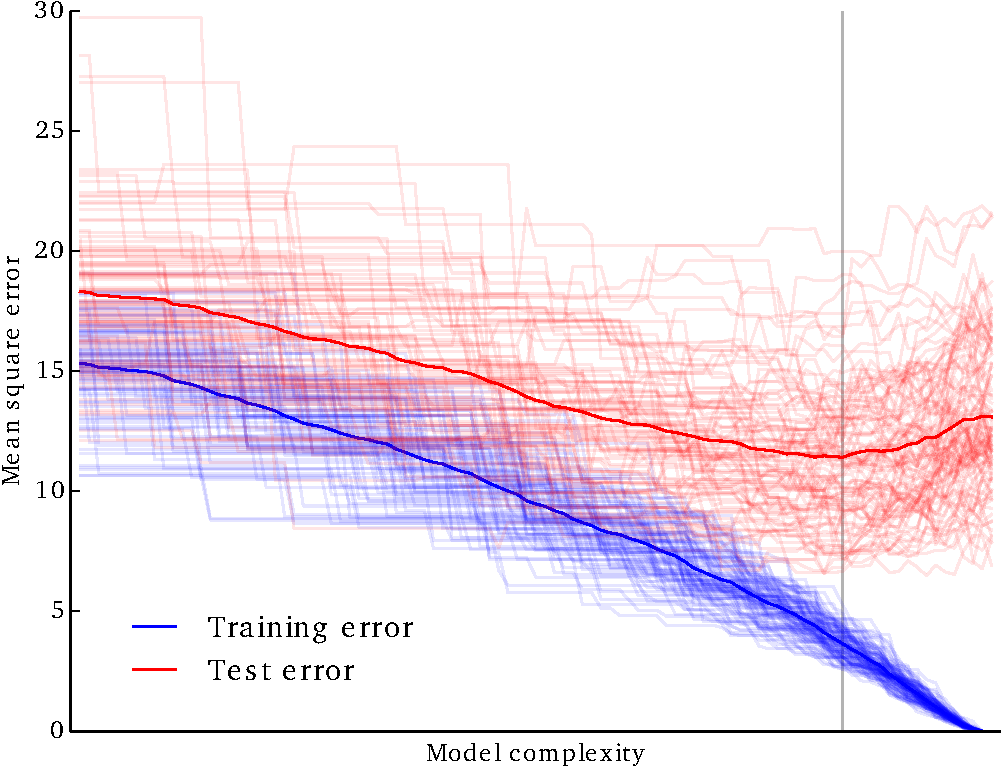
\includegraphics[width=0.9\textwidth]{figures/ch2_train_test_error.pdf}
    \caption{Training and test error with respect to the complexity
             of a model. The light blue curves show the training error over
             ${\cal L}_\text{train}$ while the light red curves show the test
             error estimated over ${\cal L}_\text{test}$ for $100$ pairs of training
             and test sets ${\cal L}_\text{train}$ and ${\cal L}_\text{test}$
             drawn at random from a known distribution. The thick blue curve
             is the average training error while the thick red curve is the
             average test error. (Figure inspired from \citep{hastie:2005}.) }
    \label{fig:train-test-error}
\end{figure}

As Figure~\ref{fig:train-test-error} illustrates, this phenomenon can be
observed by examining the respective training and test estimates of the model
with respect to its complexity\footnote{Unless mentioned otherwise, {\it
complexity} here refers to the complexity of the model in function space. {\it
Computational complexity} is studied later in
Section~\ref{sec:5:complexity-fit}}. When the model is too simple, both the training and test estimates are
large because of underfitting. As complexity increases, the model gets more
accurate and both the training and test estimates decrease. However, when the
model becomes too complex, specific elements from the training set get
captured, reducing the corresponding training estimates down to $0$, as if the
model were perfect. At the same time, the test estimates become worse because
the structure learned from the training set is actually too specific and does
not generalize. The model is overfitting. The best hyper-parameter value
$\theta$ is therefore the one making the appropriate trade-off and producing a
model which is neither too simple nor to complex, as shown by the gray line on
the figure.

As we will see later in Chapter~\ref{ch:forest},
overfitting can also be explained by decomposing the generalization error
in terms of bias and variance. A model which is too simple usually has
high bias but low variance, while a model which is too complex usually has
low bias but high variance. In those terms, finding the best model amounts
to make the appropriate \textit{bias-variance trade-off}.

\subsection{Selecting and evaluating simultaneously}
On real applications, and in particular when reporting results, it usually
happens that one wants to do both model selection and model assessment. That
is, having chosen a final model ${\cal A}(\widehat{\theta}^*, {\cal L})$, one
wants to also estimate its generalization error.

A naive assessment of the generalization error of the selected model might be
to simply use the test sample estimate $\smash{\widehat{Err}^\text{test}
({\cal A}(\widehat{\theta}^*, {\cal L}))}$ (i.e., $\overline{E}({\cal
A}(\widehat{\theta}^*, {\cal L}_\text{train}), {\cal L}_\text{test})$) that was
minimized during model selection. The issue with this estimate is that the
learned model is not independent from ${\cal L}_\text{test}$ since its repeated
construction was precisely guided by the minimization of the prediction error
over ${\cal L}_\text{test}$. As a result, the minimized test sample error is in
fact a biased, optimistic, estimate of the true generalization error, sometimes
leading to substantial underestimations. For the same reasons, using the $K$-fold
cross-validation estimate does not provide a better estimate since model
selection was similarly guided by the minimization of this quantity.

To guarantee an unbiased estimate, the test set on which the generalization
error is evaluated should ideally be kept out of the entire model selection
procedure and only be used once the final model is selected.
Algorithm~\ref{algo:train-valid-test} details such a protocol. Similarly,
per-fold estimates of the generalization error should be kept out of the model
selection procedure, for example using nested cross-validation within each
fold, as explicited in Algorithm~\ref{algo:cv}.

\begin{algorithm}\label{algo:train-valid-test}
Train-Valid-Test set protocol for both model selection and evaluation.

\begin{enumerate}
\item Divide the learning set ${\cal L}$ into three parts
      ${\cal L}_\text{train}$, ${\cal L}_\text{valid}$ and ${\cal L}_\text{test}$;
\item Perform model selection on ${\cal L}_\text{train} \cup {\cal L}_\text{valid}$
      using test sample estimates, i.e., find:
      \begin{align}
      \widehat{\theta}^* &= \argmin_{\theta} \widehat{Err}^\text{test}({\cal A}(\theta, {\cal L}_\text{train} \cup {\cal L}_\text{valid})) \\
                         &= \argmin_{\theta} \overline{E}({\cal A}(\theta, {\cal L}_\text{train}), {\cal L}_\text{valid});
      \end{align}
\item Evaluate the (unbiased) generalization error of the final model as
      \begin{equation}
      \overline{E}({\cal A}(\widehat{\theta}^*, {\cal L}_\text{train} \cup {\cal L}_\text{valid}), {\cal L}_\text{test});
      \end{equation}
\item Learn the final model ${\cal A}(\widehat{\theta}^*, {\cal L})$ on the entire learning set.
\end{enumerate}
\end{algorithm}

\begin{algorithm}\label{algo:cv}
Nested $K$-fold cross-validation protocol for both model selection and evaluation.

\begin{enumerate}
\item Divide the learning set ${\cal L}$ into $K$ folds ${\cal L}_1, ..., {\cal L}_K$;
\item For each fold $k=1, ..., K$:
    \begin{enumerate}
        \item Divide ${\cal L}\setminus{\cal L}_k = {\cal L}^{-k}$ into $K$ folds ${\cal L}_1^{-k}, ..., {\cal L}_K^{-k}$;
        \item Perform model selection on the subset ${\cal L}^{-k}$ using nested $K$-fold estimates, i.e., find:
        \begin{align}
            \widehat{\theta}_k^* &= \argmin_{\theta} \widehat{Err}^{CV}({\cal A}(\theta, {\cal L}^{-k}))\\
                                 &= \argmin_{\theta} \frac{1}{K} \sum_{l=1}^K \overline{E}({\cal A}(\theta, {\cal L}^{-k} \setminus {\cal L}_l^{-k}), {\cal L}_l^{-k});
        \end{align}
        \item Evaluate the generalization error of the selected sub-model as
        \begin{equation}
            \overline{E}({\cal A}(\widehat{\theta}^*_k, {\cal L}\setminus{\cal L}_k), {\cal L}_k);
        \end{equation}
    \end{enumerate}
\item Evaluate the (unbiased) generalization error of the selected model as the average generalization estimate of the sub-models selected over the folds:
\begin{equation}
\frac{1}{K} \sum_{k=1}^K \overline{E}({\cal A}(\widehat{\theta}^*_k, {\cal L}\setminus{\cal L}_k), {\cal L}_k);
\end{equation}
\item Perform model selection on the entire learning set ${\cal L}$ using $K$-fold cross-validation estimates, i.e., find:
\begin{align}
    \widehat{\theta}^* &= \argmin_{\theta} \widehat{Err}^{CV}({\cal A}(\theta, {\cal L}))\\
                       &= \argmin_{\theta} \frac{1}{K} \sum_{k=1}^K \overline{E}({\cal A}(\theta, {\cal L} \setminus {\cal L}_k), {\cal L}_k);
\end{align}
\item Learn the final model ${\cal A}(\widehat{\theta}^*, {\cal L})$ on the entire learning set.
\end{enumerate}
\end{algorithm}


\section{Classes of learning algorithms}
\label{sec:2:classes-of-algorithms}

Before proceeding in the next chapters, and for the rest of this work, to an
in-depth analysis of the class of tree-based methods,  we briefly review in
this section some of the other learning algorithms that have matured in the
field, including linear methods, support vector machines, neural networks and
nearest neighbor methods.

\subsection{Linear methods}

One of the oldest class of supervised learning algorithms is the class of
\textit{linear methods} from the field of statistics. In these methods, the central
assumption made on ${\cal H}$ is that the output variable $Y$ can be described
as a linear combination of the input variables $X_1, ..., X_p$ (i.e., as an hyperplane), or at least
that the linear model is a reasonable approximation. For regression, ${\cal H}$
includes all models $\varphi$ of the form:
\begin{equation}
\varphi(\mathbf{x}) = b + \sum_{j=1}^p x_j w_j
\end{equation}
For binary classification (i.e., when ${\cal Y}=\{c_1, c_2\}$),  ${\cal H}$ includes all
models $\varphi$ of the form:
\begin{equation}\label{eqn:linear-model}
\varphi(\mathbf{x}) = \begin{cases}
c_1 & \text{if } b + \sum_{j=1}^p x_j w_j > 0\\
c_2 & \text{otherwise}
\end{cases}
\end{equation}

Linear methods come in many flavors but mostly differ from each other in the
way they estimate the coefficients $b$ and $w_j$ (for $j=1,\dots,p$), usually
using some specific optimization procedure to minimize a specific criterion.
Among all of them, the most famous is the method of \textit{least squares}. It
consists in finding the $b$ and $w_j$ coefficients that minimize the
resubstitution estimate (Equation~\ref{eqn:training-error}) using the squared
error loss.

Despite an apparent simplicity, linear methods often provide reliable
predictions and an interpretable description of how the input variables affect
the output. Contrary to their name, linear methods can also be used to model
non-linear relations between $X$ and $Y$, for example by applying these methods
on (non-linear) transformations of the input variables. For more details on
(generalized) linear methods, see the reviews of \citet{maccullagh:1989},
\citet{hastie:2005}, \citet{bishop:2006} or \citet{duda:2012}.


\subsection{Support vector machines}

When data points from the learning set are linearly separable, there exist
several hyperplanes (i.e., several linear models) that are in fact equally as
good when evaluated in resubstitution. In generalization however, these
hyperplanes are usually not equivalent. As illustrated in
Figure~\ref{fig:hyperplane}, a good separation is intuitively achieved when the
distance (also known as the \textit{margin}) to the nearest training data
points is as large as possible, since in general the larger the margin the
lower the generalization error of the model.

\begin{figure}
    \centering
    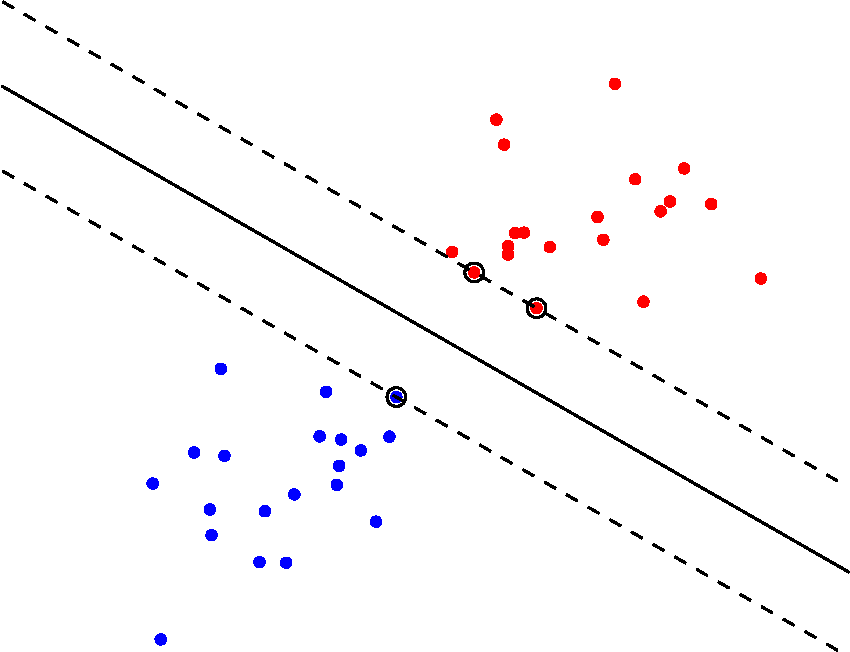
\includegraphics[width=0.9\textwidth]{figures/ch2_hyperplane.pdf}
    \caption{A good separating hyperplane is an hyperplane that maximizes the distance to the nearest training data points.}
    \label{fig:hyperplane}
\end{figure}

Mathematically, support vector machines~\citep{boser:1992,cortes:1995} are
maximum-margin linear models of the form of Equation~\ref{eqn:linear-model}.
Assuming without loss of generality that ${\cal Y}=\{-1,1\}$ and that $b=0$,
support vector machines are learned by solving the following primal
optimization problem:
\begin{equation}
\min_{\mathbf{w},\xi } \left\{\frac{1}{2} \|\mathbf{w}\|^2 + C \sum_{i=1}^N \xi_i \right\}
\end{equation}
subject to
\begin{equation}
y_i(\mathbf{w}\cdot\mathbf{x_i}) \ge 1 - \xi_i, \quad \xi_i \ge 0.
\end{equation}
In its dual the form, the optimization problem is
\begin{equation}
\max_{\alpha} \left\{ \sum_{i=1}^N \alpha_i - \frac{1}{2}\sum_{i, j} \alpha_i \alpha_j y_i y_j \mathbf{x}_i\cdot\mathbf{x}_j \right\}
\end{equation}
subject to
\begin{equation}
0 \leq \alpha_i \leq C,
\end{equation}
where $C$ is an hyper-parameter that controls
the degree of misclassification of the model, in case classes are not linearly
separable. From the solution of dual problem, we have
\begin{align}
\textbf{w} = \sum_{i=1}^N \alpha_i y_i \mathbf{x}_i,
\end{align}
from which the final linear model can finally be expressed.

Support vector machines extend to non-linear classification by projecting the
original input space into a high-dimensional space (the so-called
\textit{kernel trick}), where a separating hyperplane can hopefully be found.
Interestingly, the dual optimization problem is exactly the same, except that
the dot product $\mathbf{x}_i\cdot\mathbf{x}_j$ is replaced by a
\textit{kernel} $K(\mathbf{x}_i, \mathbf{x}_j)$\label{ntn:kernel}, which
corresponds the dot product of $\mathbf{x}_i$ and $\mathbf{x}_j$ in the new
space.


\subsection{Neural networks}

The family of \textit{neural networks} methods finds its origins in attempts to
identify mathematical representations of information processing in biological
systems. While this objective is still far from being reached, (artificial)
neural networks have nonetheless proven all their worth from a statistical point of
view, and have actually grown into one of the most effective methods in machine
learning.

A neural network is usually made of several units, also known as \textit{neurons}, of the form
\begin{equation}
h_j(\mathbf{x}) = \sigma(w_j + \sum_{i=1}^n w_{ij} x_i),
\end{equation}
where $\sigma$ is a non-linear activation function, such as the sign function,
the sigmoid function or the softmax activation. In most cases, these units are
structured into successive layers, where the outputs of a layer are directed
through weighted connections, also known as \textit{synapses}, to the inputs of
the next layer. As an example, Figure~\ref{fig:mlp} illustrates a three layered
neural network. The first layer is the input layer, which transmits the input
values $\mathbf{x} = (x_1, ..., x_p)$ to the second layer. The second layer is
made of activation units $h_j$, taking as inputs the weighted values of the
input layer and producing non-linear transformations as outputs. The third
layer is made of a single activation unit, taking as inputs the weighted
outputs of the second layer and producing the predicted value $\hat{y}$.
Assuming that this structure is fixed and that all units from the network make
use of the same activation function $\sigma$, the hypothesis space ${\cal H}$
therefore includes all models $\varphi$ of the form
\begin{equation}
\varphi(\mathbf{x}) = \sigma(w_5 + \sum_{j=1}^4 w_{j5} \sigma(w_j + \sum_{i=1}^p w_{ij} x_i)).
\end{equation}

\begin{figure}
    \centering
    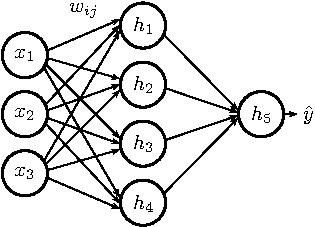
\includegraphics[scale=1.0]{figures/ch2_mlp.pdf}
    \caption{An artificial neural network.}
    \label{fig:mlp}
\end{figure}

As for linear methods, learning a neural network  amounts to estimate the
weights $w_{ij}$ that minimize some specific loss function, using some specific
optimization procedure. Among all of them, the most famous is the
\textit{backpropagation algorithm}~\citep{bryson:1975}.

Recent advances on neural networks, now themed as \textit{deep learning}, have
recently shown the capability of these models to autonomously learn high-level
and very effective representations of data. On various difficult tasks, such as
image classification or speech recognition, neural networks have indeed
achieved outstanding performance, outperforming both human operators and
state-of-the-art methods. From a theoretical point of view however, little is
still known about what makes them truly work. In particular, picking the
appropriate combination of number of units, layers and types of activation
functions remains a delicate task, which unfortunately makes (deep) neural
networks still difficult to use for non-experts. Reviews on recent developments
include the works of \citet{hinton:2007}, \citet{arel:2010} or \citet{bengio:2013}.


\subsection{Nearest neighbor methods}

\textit{Nearest neighbor methods} belong to a class of non-parametric algorithms
known as \textit{prototype methods}~\citep{hastie:2005}. They distinguish from
other learning algorithms in the sense that they are memory-based and require
no model to be fit.

The principle behind nearest neighbor methods is to find a number of
training samples closest in distance to the new sample, and then infer from
these the value of the output variable. For regression, the $k$-nearest
neighbor algorithm~\citep{fix:1951} averages the output values from the $k$
closest training samples, that is:
\begin{equation}
\varphi(\mathbf{x}) = \frac{1}{k} \sum_{(\mathbf{x_i}, y_i) \in NN(\mathbf{x}, {\cal L}, k)} y_i,
\end{equation}
where $NN(\mathbf{x}, {\cal L}, k)$ denotes the $k$ nearest neighbors of ${\mathbf{x}}$ in ${\cal L}$.
For classification, the procedure is the same except that the predicted
output value is computed as the majority class among the $k$ nearest neighbors:
\begin{equation}
\varphi(\mathbf{x}) = \argmax_{c \in {\cal Y}} \sum_{(\mathbf{x_i}, y_i) \in NN(\mathbf{x}, {\cal L}, k)} 1(y_i = c).
\end{equation}
In general, the distance function used to identify the $k$ nearest neighbors
can be any metric, but the standard Euclidean distance is the most common
choice. A notable variant is the
\textit{radius-based neighbor algorithm}, in which the predicted output value
is computed from the training samples within a radius $r$ of the new sample.
In cases where data is not uniformly sampled, this latter algorithm can be
a better choice than the $k$-nearest neighbor method.

Despite their simplicity, nearest neighbor methods usually yield decent
results in practice. They are are often successful in classification situations
where the decision boundary is very irregular. From a theoretical point of
view, an important result due to \citet{cover:1967} is the proof of consistency
of the method. When the size of ${\cal L}$ tends to infinity and $k$ is
appropriately adjusted to ${\cal L}$, the generalization error of the model
produced by the $k$-nearest neighbor method is shown to converge towards the
generalization error of the Bayes model.

\section{预备知识}

\subsection{Bayesian Personalized Ranking}
\begin{figure}[htbp]
	% caption放上面就会显示在图的上方,出现在下面就是出现在图的下方
	% label的位置也有讲究
	\begin{center}
		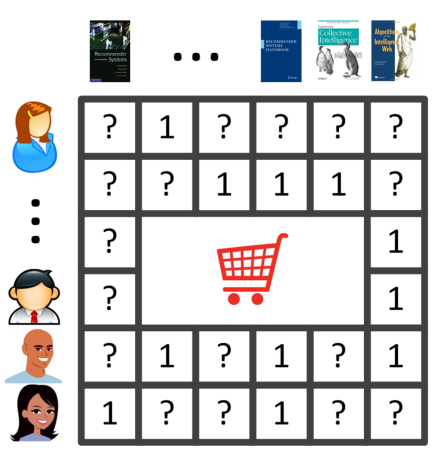
\includegraphics[width=3in]{matrix}
		\caption{user-item 隐式反馈矩阵}
		\label{gra3}
	\end{center}
\end{figure}
在这一节, 我们首先回顾BPR算法,然后讨论它的一些局限性,也就是其收敛缓慢与冷启动问题。通常用户与物品的隐式反馈可以表示为如图\ref{gra3}所示的矩阵, 矩阵的“1”表示用户已经对该物品有过交互行为, 比如购买,点击等, 矩阵的“?”则表示用户还未对该物品有过交互行为。

\subsubsection{Pairwise Preference Assumption}
BPR\cite{rendle2009bpr}是一个应对隐式反馈很流行的推荐框架. 它基于这样一个偏好假设: 如果一个用户$u$已经选择了物品$i$但是没有选择物品$j$,那么在BPR中, 我们认为相对于物品$j$用户$m$更喜欢物品$i$,并定义用户$u$关于物品$i$与$j$的偏好关系为:
\begin{equation}
\label{pairwisepre}
p \left( i \succ_u j \right) := f \left( x_{uij} \right),
\end{equation}
这里$f \left(x\right) = 1/\left(1+exp\left(-x\right)\right)$\footnote{$f \left(x\right)$即为sigmoid函数}, $x_{uij} := s\left(u,i\right) - s\left(u,j\right)$, $s\left(\cdot,\cdot\right)$可以是任何表示用户与物品相关程度的函数。在BPR\cite{rendle2009bpr}中, $s\left(\cdot,\cdot\right)$为用户对物品的预测值, 即$s\left(u,i\right) = \hat{r}_{ui}$, $x_{uij} = \hat{r}_{ui}-\hat{r}_{uj}$.


\subsubsection{预测公式}

在BPR中, 用户$u$对于物品$i$的预测值$\hat{r}_{ui}$公式为:
\begin{equation}
\hat{r}_{ui} = U_{u\cdot}V_{i\cdot}^T + b_i
\end{equation}


\subsubsection{Likelihood of Pairwise Preference}

伯努利分布(Bernouli distribution)是关于布尔变量 $x \in \{0,1\}$ 的概率分布, 其连续参数 $p \in \left[0,1\right]$的概率.
\begin{equation}
\left( x|p \right) = Ber\left(x|p \right)=p^x\left(1-p \right)^{1-x}
\end{equation}

若记事件 $\left(\hat{r}_{ui} > \hat{r}_{uj}\right)$ 的概率为$p\left(\hat{r}_{ui} > \hat{r}_{uj}\right)$, 布尔变量$\delta\left(\left(u,i\right) \succ \left(u,j\right)\right)$ 服从伯努利分布, 那么用户$u$的likelihood of pairwise preference 在\cite{rendle2009bpr}中被定义为:
\begin{equation}
\label{LPP}
\begin{aligned}
LPP_u  
&= \prod_{i,j \ \in \  \mathcal{I}}p\left(\hat{r}_{ui} > \hat{r}_{uj}\right)^{\delta\left(\left(u,i\right) \succ \left(u,j\right)\right)} \left[1-p\left(\hat{r}_{ui} > \hat{r}_{uj}\right)\right]^{1-\delta\left(\left(u,i\right) \succ \left(u,j\right)\right)}\\
&= \prod_{\left(u,i\right) \succ \left(u,j\right)}p\left(\hat{r}_{ui} > \hat{r}_{uj}\right)\prod_{\left(u,i\right) \preceq \left(u,j\right)}\left[1-p\left(\hat{r}_{ui} > \hat{r}_{uj}\right)\right]
\end{aligned}
\end{equation}

这里的$\left(u,i\right) \succ \left(u,j\right)$ 表示用户 $u$ 相比物品 $i$ 更喜欢物品 $j$.

用 $f \left(\hat{r}_{uij} \right)$ 来近似表示概率
$p\left(\hat{r}_{ui} > \hat{r}_{uj}\right)$ \cite{rendle2009bpr}, 对于公式\ref{LPP}取其对数即$\ln LPP_u$, 那么就有:
\begin{equation}
\label{eq5}
\begin{aligned}
\ln LPP_u
&= \ln \prod_{\left(u,i\right) \succ \left(u,j\right)} f \left(\hat{r}_{uij}\right) + \ln \prod_{\left(u,i\right) \preceq \left(u,j\right)}\left[1- f \left(\hat{r}_{uij}\right)\right]\\
&= \ln \prod_{\left(u,i\right) \succ \left(u,j\right)} f \left(\hat{r}_{uij}\right) + \ln \prod_{\left(u,i\right) \succ \left(u,j\right)}\left[1-\left(1- f \left(\hat{r}_{uij}\right)\right)\right]\\
&= \ln \prod_{\left(u,i\right) \succ \left(u,j\right)} f \left(\hat{r}_{uij}\right) + \ln \prod_{\left(u,i\right) \succ \left(u,j\right)} f \left(\hat{r}_{uij}\right)\\
&= 2\ln \prod_{\left(u,i\right) \succ \left(u,j\right)} f \left(\hat{r}_{uij}\right)\\
&= 2 \sum_{i\in\mathcal{I}_u^{tr}}
\sum_{j \in \mathcal{I}\setminus \mathcal{I}_u^{tr}}\ln f \left(\hat{r}_{uij}\right)
\end{aligned}
\end{equation}
在这里$\hat{r}_{uij} = \hat{r}_{ui} - \hat{r}_{uj}$, $f \left(x\right) = 1/\left(1+exp\left(-x\right)\right)$, .

\subsubsection{目标函数}

基于上面的成对偏好假设,可以从隐式反馈数据集中得到所有的偏好集合$D_S := \{\left(u,i,j\right) | v_i \in I_{u}^+ \wedge v_j \in I \setminus I_{u}^+\}$,$I_m^+$表示被用户$u$选择过的物品集合,三元组$\left(u,i,j\right)$表示用户$u$选择过物品$v_i$但是没有选择过物品$v_j$。我们把$v_i$叫做一个positive item,$v_j$叫做一个negative item。对于给定的集合$D_S$, BPR的目标便是最大化所有user-item pair的似然偏好:

\begin{equation}
\label{eq6}
arg \max_{\substack \Theta } \prod_{\left(u,i,j\right) \in D_S} p\left(i \succ_u j\right),
\end{equation}

公式\eqref{eq6}等价于最小化负的对数似然函数:

\begin{equation}
\label{Lfeedback}
L_{feedback} = - \sum_{\left(u,i,j\right) \in D_S}\ln f \left( x_{uij}\right) + \lambda\|\Theta\|^2,
\end{equation}
这里的$x_{uij} = \hat{r}_{uij}$, $\Theta$表示算法中需要学习的模型参数集合,$\lambda$表示超参数集合。在实际的算法学习中, BPR的学习算法经常采用均匀采样的随机梯度下降(\textbf{S}tochastic \textbf{G}radient \textbf{D}escent)进行迭代学习。

更为具体的,公式\eqref{Lfeedback}也就是最小化下面的目标函数(Objective Function): 
\begin{equation}
\label{eq8}
\min_{\substack\Theta}\sum_{u\in\mathcal{U}} \ \sum_{i\in\mathcal{I}_u}\sum_{j\in\mathcal{I}\setminus\mathcal{I}_u}\Phi_{uij}
\end{equation}
这里的
$\Phi_{uij}
= 
- \ln f \left(\hat{r}_{uij}\right) 
+ \frac{\alpha_u}{2}\|U_{u\cdot}\|^2
+ \frac{\alpha_v}{2}\|V_{i\cdot}\|^2
+ \frac{\alpha_v}{2}\|V_{j\cdot}\|^2
+ \frac{\beta_v}{2}\|b_{i}\|^2
+ \frac{\beta_v}{2}\|b_{j}\|^2$, $\Theta = \{U_{u\cdot},V_{i\cdot},b_i\}
$的将要学习的参数集合。


\subsubsection{随机梯度}
对于一个随机采样而得的三元组$\left(u,i,j\right)$, 对目标函数中的参数求其偏导即可得梯度。

在此之前先做一些准备工作,对于函数$f(x) = 1/\left(1+e^{-x}\right)$的导数:

\begin{equation*}
f^{'}(x) = -\frac{1}{\left(1+e^{-x}\right)^2} e^{-x}\left(-1\right) = \frac{e^{-x}}{\left(1+e^{-x}\right)^2} = \frac{1}{\left(1+e^{x}\right)\left(1+e^{-x}\right)} = {f(x)f(-x)}
\end{equation*}

下面开始对参数$U_{u\cdot}$求其偏导:
\begin{equation}
\begin{aligned}
\bigtriangledown U_{u\cdot} 
= \frac{\partial \Phi_{uij}}{\partial U_{u\cdot}}
&=-\frac{\partial \ln f\left(\hat{r}_{uij}\right)}{\partial f\left(\hat{r}_{uij}\right)} 
\frac{\partial f\left(\hat{r}_{uij}\right) }{\partial \hat{r}_{uij}} 
\frac{\partial \hat{r}_{uij}}{\partial U_{u\cdot}}
\ + \  \alpha_uU_{u\cdot}\\
&= -\frac{1}{f\left(\hat{r}_{uij}\right)} 
\frac{\partial f\left(\hat{r}_{uij}\right) }{\partial \hat{r}_{uij}} 
\frac{\partial \hat{r}_{uij}}{\partial U_{u\cdot}}
\ + \  \alpha_uU_{u\cdot}\\
&= -\frac{1}{f\left(\hat{r}_{uij}\right)} 
{f\left(\hat{r}_{uij}\right) f\left(-\hat{r}_{uij}\right)}
\frac{\partial f\left(\hat{r}_{ui} - \hat{r}_{uj}\right) }{\partial U_{u\cdot}} 
\ + \ \alpha_uU_{u\cdot}\\
&= -{f\left(-\hat{r}_{uij}\right)} \frac{\partial f\left[\left(U_{u\cdot}V_{i\cdot}^T+b_i\right) - \left(U_{u\cdot}V_{j\cdot}^T+b_j\right)\right] }{\partial U_{u\cdot}} 
\ + \ \alpha_uU_{u\cdot}\\
&= -{f\left(-\hat{r}_{uij}\right)} \left(V_{i\cdot} - V_{j\cdot}\right)  
\ + \  \alpha_uU_{u\cdot}\\
\end{aligned}
\end{equation}

同样其他参数随机梯度如下:
%\begin{equation}
\begin{align} %align环境不要有空行
\bigtriangledown V_{i\cdot} &= \frac{\partial \Phi_{uij}}{\partial V_{i\cdot}}=-f\left(-\hat{r}_{uij}\right)U_{u\cdot} + \alpha_vV_{i\cdot}\\
\bigtriangledown V_{j\cdot} &= \frac{\partial \Phi_{uij}}{\partial V_{j\cdot}}=-f\left(-\hat{r}_{uij}\right)\left(-U_{u\cdot}\right) + \alpha_vV_{j\cdot}\\
\bigtriangledown b_i        &= \frac{\partial \Phi_{uij}}{\partial b_i} =-f\left(-\hat{r}_{uij}\right)+\beta_vb_i\\
\bigtriangledown b_j        &= \frac{\partial \Phi_{uij}}{\partial b_j} =-f\left(-\hat{r}_{uij}\right)\left(-1\right)+\beta_vb_j
\end{align}
%\end{equation}

\subsubsection{迭代更新}
对于三元组  $\left(u,i,j\right)$ 在采用SGD的BPR算法中的更新公式如下:
%align环境的每行公式默认会进行编号,aligned环境不会
\begin{align}
	\label{eq10}
U_{u\cdot} &= U_{u\cdot} - \gamma\bigtriangledown U_{u\cdot}\\
V_{i\cdot} &= V_{i\cdot} - \gamma\bigtriangledown V_{i\cdot}\\
V_{j\cdot} &= V_{i\cdot} - \gamma\bigtriangledown V_{j\cdot}\\
b_{i\cdot} &= b_i - \gamma\bigtriangledown b_{i}\\
b_{j\cdot} &= b_j - \gamma\bigtriangledown b_{j}
\end{align}

这里的 $\gamma$ 为学习率(learning rate).

\subsubsection{BPR算法}
如算法\ref{al1}即为采用SGD求解的BPR算法。
\IncMargin{1em}
\begin{algorithm}[ht]
	\SetAlgoNoLine %不要算法中的竖线
	\BlankLine
	
	initialize the model parameter $\Theta$\;
	\For {$t_1 = 1,\cdots,T$}{
		\For {$t_2 = 1,\cdots, |\mathcal{P}|$}{
			Randomly pick up a pair $\left(u,v_i\right) \in \mathcal{P}$\;
			Randomly pick up an item $v_j$ from $\mathcal{I} \setminus \mathcal{I}_{u}^+$\;
			Calculate the gradients via Eq.(9-13)\;
			Update the model parameters via Eq.(14-18)\;
		}	
	}
	\caption{The SGD algorithm for BPR}
	\label{al1}%label 放置的位置有讲究, 放后面
\end{algorithm}
\DecMargin{1em}

\subsubsection{收敛缓慢的原因}
由于上面的均匀采样方式会产生很多对于参数学习贡献微弱的train pairs,因此常常会导致收敛缓慢。确切的讲,对于一个给定的训练采样$\left(u,i,j\right) \in D_S$, 由公式\ref{Lfeedback}对随机梯度下降的任意一参数$\theta \in \Theta$求其偏导:

\begin{equation}
\label{eq19}
\frac {\partial L_{feedback}} {\partial\theta} 
= -f\left(-x_{uij}\right)\frac{\partial\left(x_{uij}\right)}{\partial\theta}
= \left(f\left(x_{uij}\right)-1\right) \frac{\partial\left(x_{uij}\right)}{\partial\theta}
\end{equation}

根据公式\eqref{eq19},如果$f \left(x_{uij}\right) \rightarrow +1$,随机梯度将接近于0,则训练采样$\left(u,i,j\right)$对于优化目标的贡献将会变得很小。
\begin{figure}[htbp]
	\begin{center}
		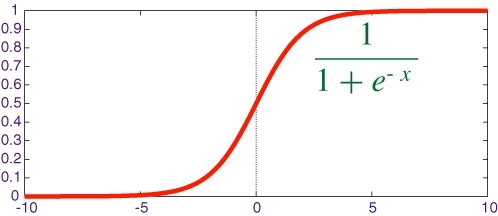
\includegraphics[width=4in]{sigmoid}
		\caption{sigmoid函数$f \left(x\right) $图像}
		\label{gra-sigmoid}
	\end{center}
\end{figure}

联系公式\eqref{eq19}与公式\eqref{pairwisepre},由图\ref{gra-sigmoid} sigmoid函数图像可得, 当$f \left(x_{uij}\right) \rightarrow +1$时, 也就是$x_{uij} = \hat{r}_{ui} - \hat{r}_{uj}$越来越大, 即用户对于物品$v_i$与$v_j$的预测差值越来越大. 因此为了加速学习, 针对一个已有的user-item pair中的物品 $v_i$,要采样的物品$v_j$应当是$v_i$相比有竞争力的物品, 更进一步说也就是由该用户对于$v_i$与$v_j$的偏好得分应该是相近的,否则这个采样对于SGD便是低效的采样。

从经验上来讲,每个用户只会浏览一小部分的物品并对这些浏览过的物品提供一些交互反馈。如果均匀采样器均等地从整个物品集合中采样negative  item.对于一个user-item  pair,大部分均匀采样的物品并不具有可比性或者很难被相关的用户浏览。举个例子,iPhone与牙刷或iPhone与一个冷门的手机品牌可能会经常被均匀采样器采得。而由于这些低效的training pair对于SGD几乎作用很小,整个训练过程便会收敛地极其缓慢。

除此以外,与经典的分解技术相似,如果一个用户或物品缺乏足够的反馈,其对应的隐式表达往往不能够被很好的学习到。在现实世界数据集中,用户行为与物品流行度的分布往往呈现长尾状。这就导致了大部分的用户和物品仅仅有很小部分的反馈数据。此外,在真实的推荐系统中,新的个体可能在任何时间被加入到推荐系统中。因此,BPR框架也很容易受制于冷启动问题。

\subsection{Latent Dirichlet Allocation}
Latent Dirichlet allocation(LDA),隐含狄利克雷分布,是一种主题模型(topic model),它可以将文档集中每篇文档的主题按照概率分布的形式给出。同时它是一种无监督学习算法,在训练时不需要手工标注的训练集,需要的仅仅是文档集以及指定主题的数量即可。此外LDA的另一个优点则是,对于每一个主题均可找出一些词语来描述它。

LDA首先由于2003年提出\cite{blei2003latent},目前在文本挖掘领域包括文本主题识别、文本分类以及文本相似度计算方面都有应用。


\subsubsection{数学模型}
LDA是一种典型的词袋(Bag-of-words)模型,即它认为一篇文档(document)是由一组词(word)构成的一个集合,词与词之间没有顺序以及先后的关系。一篇文档可以包含多个主题(topic),文档中每一个词都由其中的一个主题生成。

\begin{figure}[htbp]
	% caption放上面就会显示在图的上方,出现在下面就是出现在图的下方
	% label的位置也有讲究
	\begin{center}
		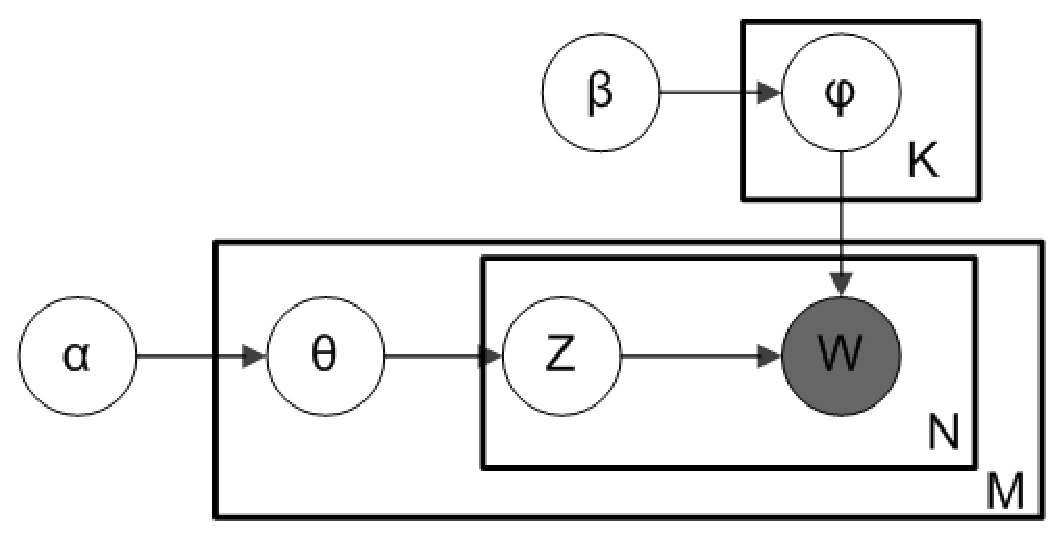
\includegraphics[width=4in]{LDA}
		\caption{LDA 贝叶斯网络结构}
		\label{gra4}
	\end{center}
\end{figure}

另外,正如Beta分布是二项式分布的共轭先验概率分布,狄利克雷分布作为多项式分布的共轭先验概率分布。因此正如图\ref{gra4}, LDA贝叶斯网络结构中所描述的,在LDA模型中一篇文档生成的方式如下:
\begin{itemize}
	\item 从狄利克雷分布$\alpha$ 中取样生成文档$i$的主题分布$\theta_i$
	\item 从主题的多项式分布$\theta_i$中取样生成文档$i$第$j$个词的主题$z_{i, j}$
	\item 从狄利克雷分布$\beta $中取样生成主题$z_{i, j}$的词语分布$\phi_{z_{i, j}}$
	\item 从词语的多项式分布$\phi_{z_{i, j}}$中采样最终生成词语$w_{i, j}$
\end{itemize}
因此整个模型中所有可见变量以及隐藏变量的联合分布是
\begin{equation}
p(w_i, z_i, \theta_i, \Phi | \alpha, \beta) = \prod_{j = 1}^{N} p(\theta_i|\alpha)p(z_{i, j}|\theta_i)p(\Phi|\beta)p(w_{i, j}|\theta_{z_{i, j}})
\end{equation}


最终一篇文档的单词分布的最大似然估计可以通过将上式的$\theta_i$以及$\Phi$进行积分和对$z_i$进行求和得到
\begin{equation}
p(w_i | \alpha, \beta)  = \int_{\theta_i}\int_{\Phi }\sum_{z_i}p(w_i, z_i, \theta_i, \Phi | \alpha, \beta) 
\end{equation}


根据$p(w_i | \alpha, \beta)$ 的最大似然估计,最终可以通过吉布斯采样等方法估计出模型中的参数。


\subsubsection{使用吉布斯采样估计LDA参数}
在LDA最初提出的时候,人们使用EM算法(Expectation-maximization algorithm)进行求解,后来人们普遍开始使用较为简单的Gibbs Sampling,具体过程如下:
\begin{itemize}
	\item 首先对所有文档中的所有词遍历一遍,为其都随机分配一个主题,即$z_{m,n}=k\sim Mult(1/K)$,其中$m$表示第$m$篇文档,$n$表示文档中的第$n$个词,$k$表示主题,$K$表示主题的总数,之后将对应的$n^{\left(k\right)}_m+1$, $n_m+1$, $n^{\left(t\right)}_k+1$, $n_k+1$, 他们分别表示在$m$文档中$k$主题出现的次数,$m$文档中主题数量的和,$k$主题对应的$t$词的次数,$k$主题对应的总词数。
	\item 之后对下述操作进行重复迭代。
	\item 对所有文档中的所有词进行遍历,假如当前文档$m$的词$t$对应主题为$k$,则$n^{\left(k\right)}_m-1$, $n_m-1$, $n^{\left(t\right)}_k-1$, $n_k-1$, 即先拿出当前词,之后根据LDA中topic sample的概率分布sample出新的主题,在对应的$n^{\left(k\right)}_m$, $n_m$, $n^{\left(t\right)}_k$, $n_k$上分别$+1$。
	\begin{equation}
	p(z_i=k|z_{-i},w) \propto k(n^{(t)}_{k,-i}+\beta_t)(n_{m,-i}^{(k)}+\alpha_k)/(\sum_{t=1}^{V}n_{k,-i}^{(t)}+\beta_t)
	\end{equation}
	\item 迭代完成后输出主题--词参数矩阵$\Phi$和文档--主题矩阵$\Theta$
	\begin{align}
	\phi_{k,t}   &=(n_k^{(t)}+\beta_t)/(n_k+\beta_t)  \\
	\theta_{m,k} &=(n_m^{(k)}+\alpha_k)/(n_m+\alpha_k)
	\end{align}
\end{itemize}









\subsection{本章小结}
本章首先介绍了采用SGD求解的Bayesian Personalized Ranking(BPR)推荐算法, 并且对可能导致其收敛缓慢的均匀采样策略做了讨论。然后简要介绍了LDA模型。
\section{Experiment}
\begin{frame}{Experiment}
	
		BPR-MF\cite{rendle2009bpr} and CA-BPR\cite{DBLP:conf/webi/GuoWWT15}
	
	\begin{table}[htbp]
		\caption{Characteristics of compared methods}
		\renewcommand\arraystretch{1.3}%改变行高
		\label{tab:characteristic}
		\begin{center}
			\begin{tabular}{|c|c|c|}
				\hline
				Method   &   Content & Sampling \\
				\hline
				\renewcommand\arraystretch{1}%改变行高
				BPR-MF   &   no      & uniform  \\
				CA-BPR   &   yes     & non-uniform\\
				\hline
				
			\end{tabular}
		\end{center}
	\end{table}
\end{frame}

\begin{frame}{Experiment}
	\begin{table}[htbp]
		\caption{The performence of approaches by MAP and NDCG.}
		\label{tab:mapandndcg}
		\begin{center}
			\begin{tabular}{|c | c |c |c|c|c|}
				\hline
				BPR-MF  &   k=10 &   k=20 &    k=30&    k=40&    k=50\\
				\hline
				MAP      &  0.0879&  0.0877&  0.1043&  0.0888&  0.1074\\
				\hline
				NDCG@3   &  0.3051&  0.3545&  0.3398&  0.2491&  0.3790\\
				NDCG@5   &  0.3616&  0.4296&  0.3708&  0.2984&  0.4153\\
				NDCG@10  &  0.4120&  0.4632&  0.4010&  0.3163&  0.4458\\
				NDCG@20  &  0.4121&  0.4575&  0.4164&  0.3415&  0.4323\\
				\hline
			\end{tabular}
		\end{center}
	\end{table}
	
	\begin{table}
		
		\begin{center}
			
			\begin{tabular}{|c | c |c |c|c|c|}
				\hline
				CA-BPR  &     k=10&   k=20 &    k=30&  k=40 &   k=50  \\
				\hline
				MAP     &   0.1074&  0.1072&  0.1274&  0.1016&  0.1229\\
				\hline
				NDCG@3  &   0.3790&  0.4336&  0.4152&  0.3044&  0.4631\\
				NDCG@5  &   0.4153&  0.4752&  0.4531&  0.3646&  0.5074\\
				NDCG@10 &   0.4458&  0.5101&  0.4900&  0.3865&  0.5447\\
				NDCG@20 &   0.4323&  0.4946&  0.5088&  0.4173&  0.5282\\
				\hline
			\end{tabular}
		\end{center}
	\end{table}
\end{frame}

\begin{frame}{Experiment}
	\begin{figure}
		\begin{center}
			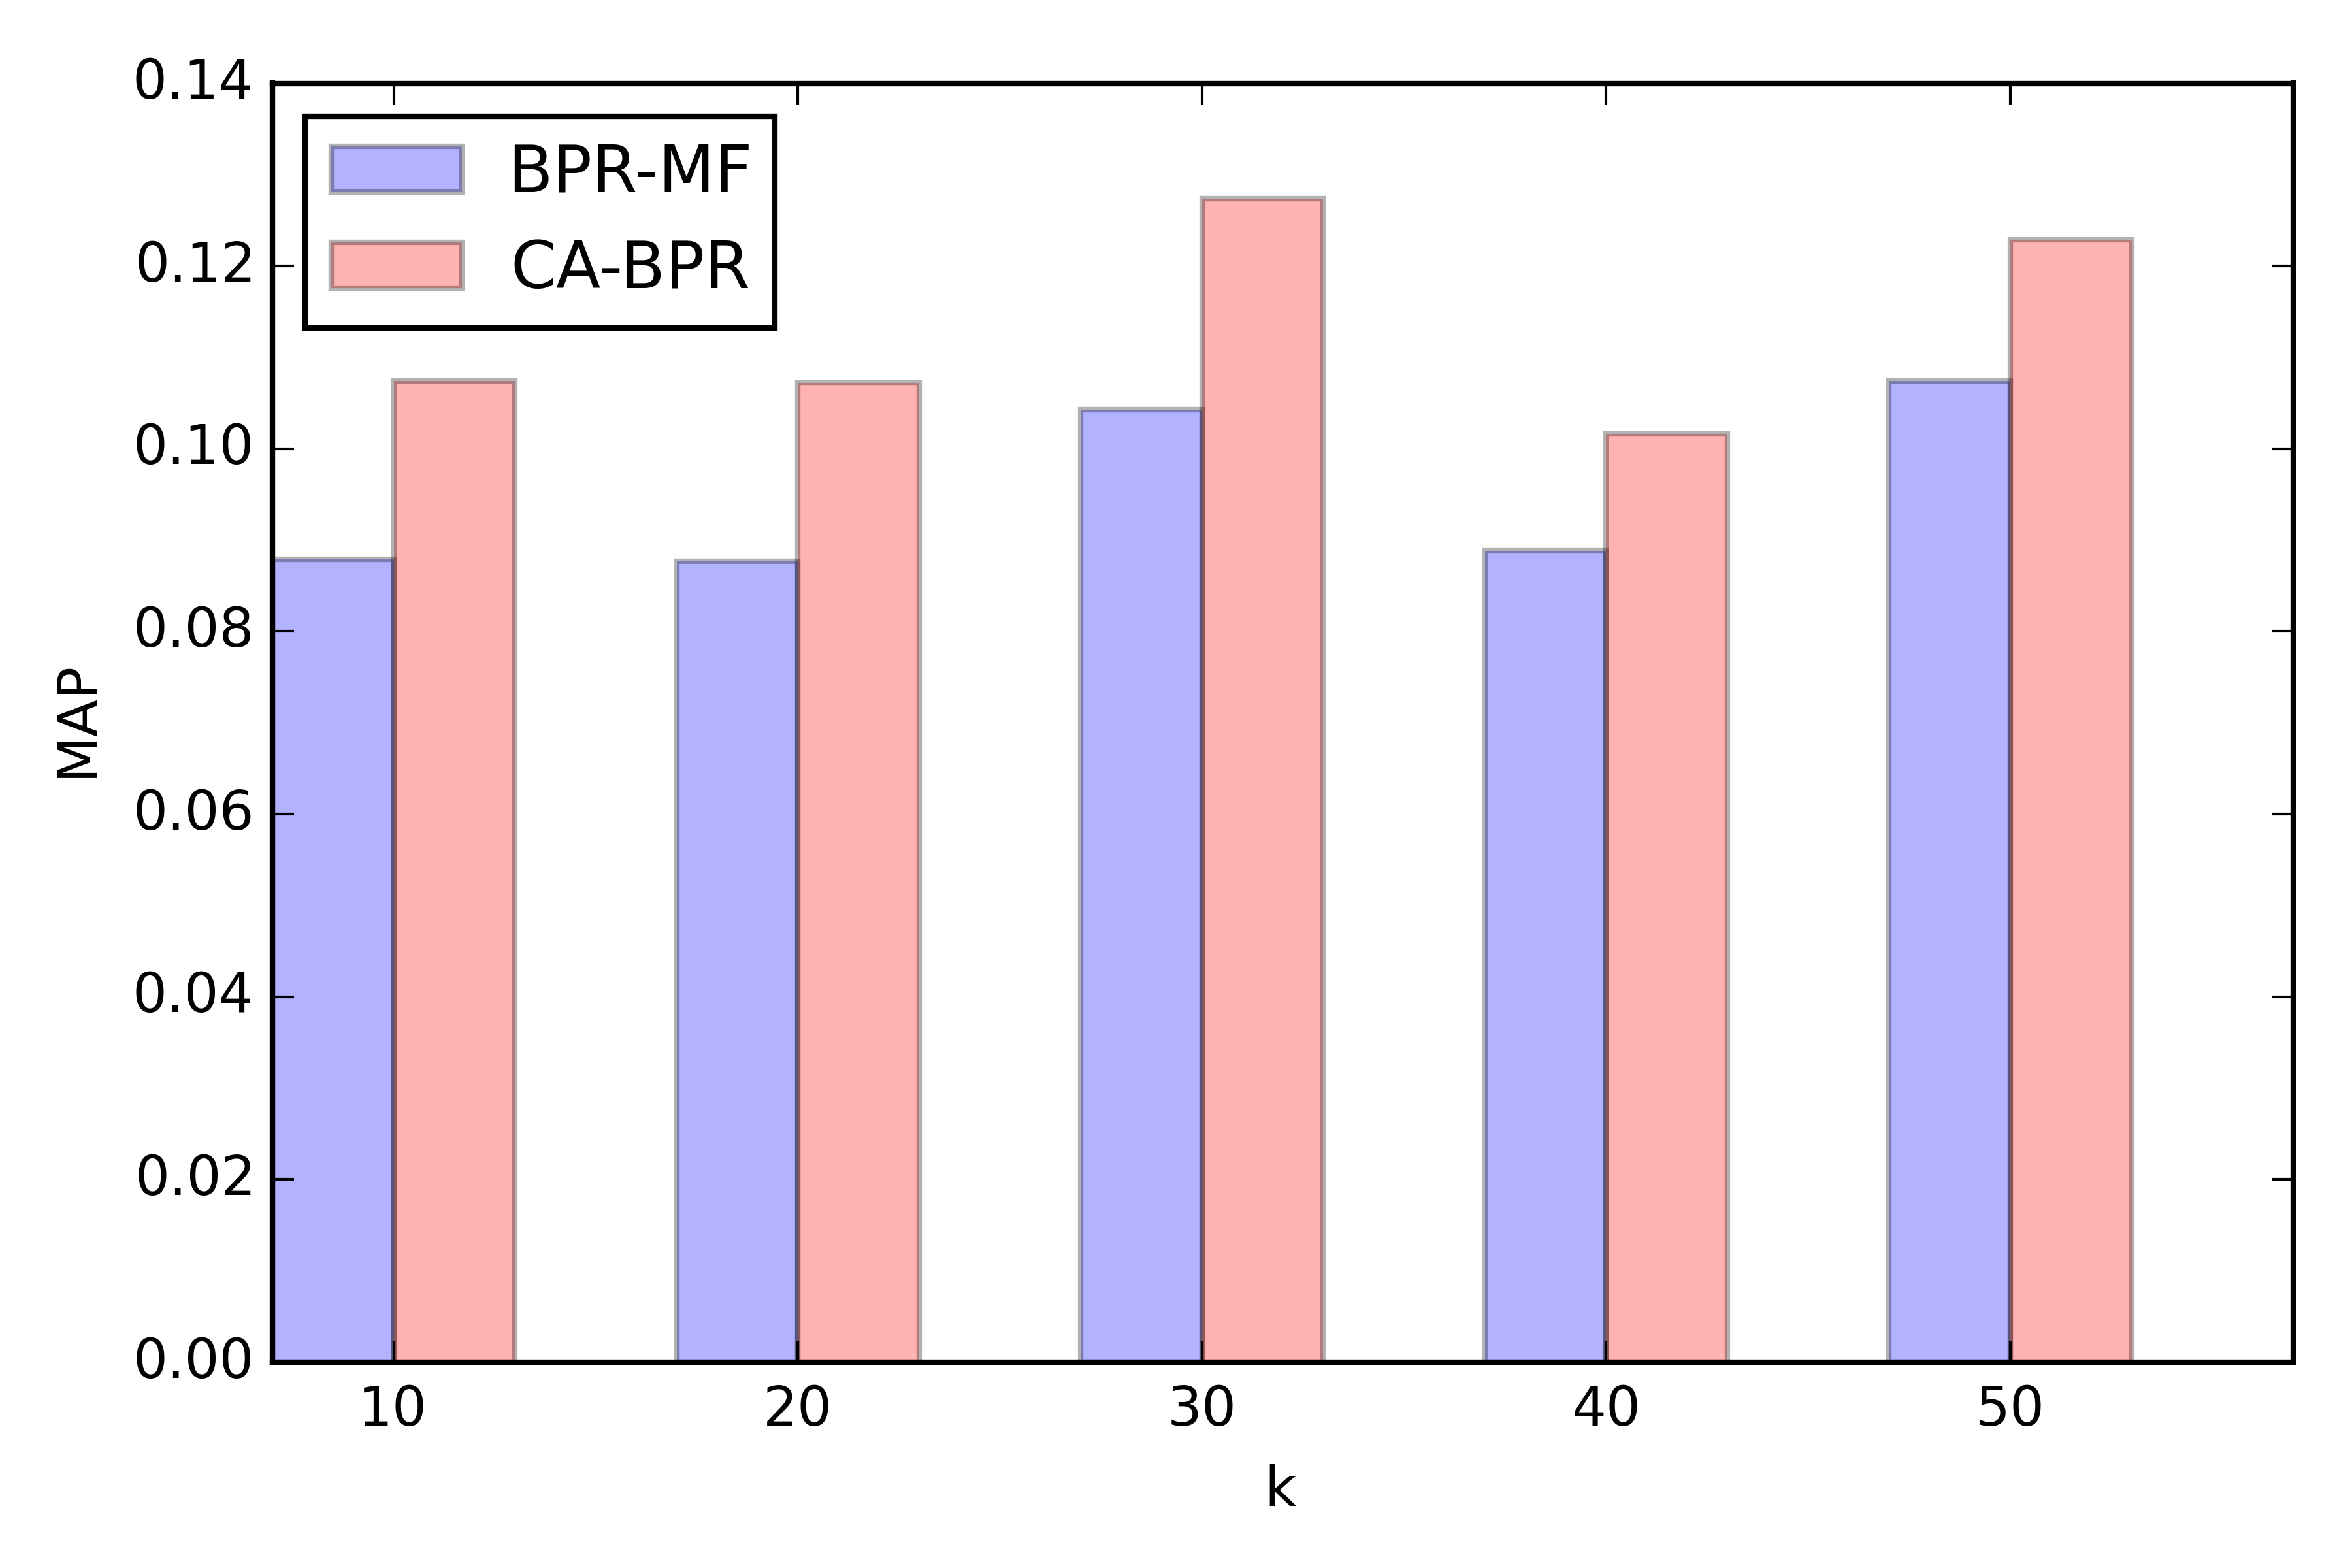
\includegraphics[width=3in]{bar}
		\end{center}
		\caption{CA-BPR indeed performs better than BPR-MF.}
	\end{figure}
\end{frame}

\begin{frame}
	\centering
	\Huge Thank you !
\end{frame}
\section{程序的使用测试}

\subsection{测试的意义及方法}

1)  测试的意义:测试的意义去检验程序中的是否存在错误,是否满足文所需要实现的签名及验证的功能。通过输入常规数据和非常规数据观察程序是否满要求。同时对测试所用数据要具有一般性,并对输入数据的有一个相应的输出期望结果,并通过对不同数据的修改观察程序是否运作正常,结果是否与期望结果一致。

2)  测试方法:先对测试用例data.txt进行签名、代理签名、验证签名及验证代理签名等操作,再改变原消息值即data.txt里的文字,再进行验证签名及验证代理签名操作,观察分析得到的结果。

\subsection{测试Elgamal签名方案}

\subsubsection{测试用例}

测试用例:1、大小为128字节的txt文档。

          2、大小为340字节的txt文档。

\subsubsection{测试过程}

1)生成公私钥对

    运行程序,根据主界面,选1,生成Elgamal公私钥对,公钥y,大素数p,本原元g保存在pub.txt;私钥x,大素数p,本原元g保存在pri.txt:

\begin{figure}[H]
\centering
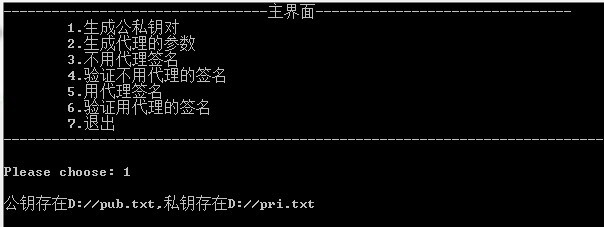
\includegraphics{img/7.jpg}
\caption{生成公私钥}
\end{figure}

Pub.txt文件中,由上至下三个大数依次为:公钥y,大素数p,本原元g

\begin{figure}[H]
\centering
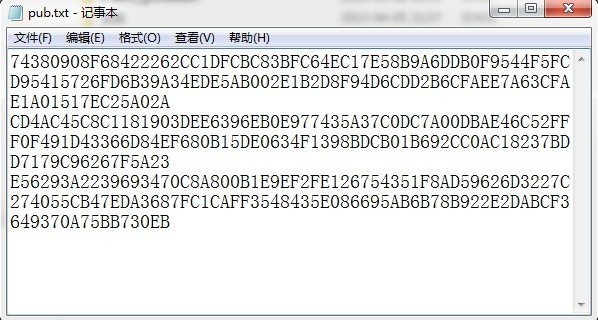
\includegraphics{img/8.jpg}
\caption{pub.txt}
\end{figure}

pri.txt,由上至下三个大数依次为私钥x,大素数p,本原元g:

\begin{figure}[H]
\centering
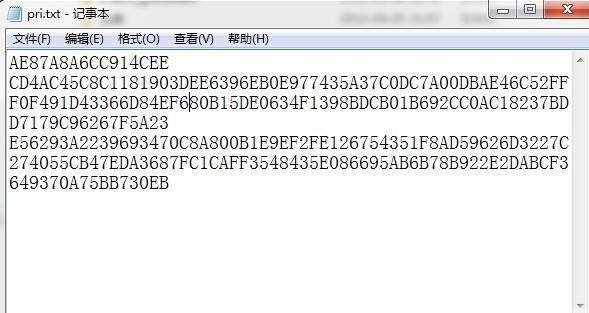
\includegraphics{img/9.jpg}
\caption{pri.txt}
\end{figure}

2)签名与验证签名
   对大小为128字节的data.txt进行签名操作,签名耗时3毫秒:

\begin{figure}[H]
\centering
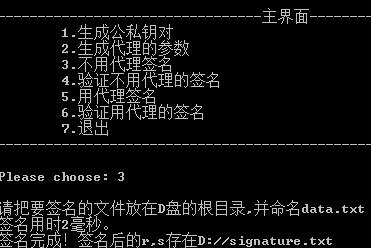
\includegraphics{img/10.jpg}
\caption{对data.txt签名}
\end{figure}

128字节的data.txt内容:

\begin{figure}[H]
\centering
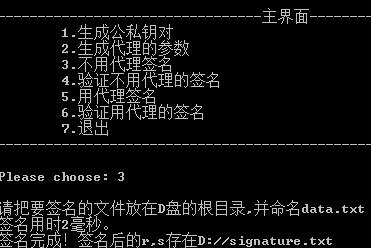
\includegraphics{img/10.jpg}
\caption{data.txt}
\end{figure}

生成的签名(r,s)保存在signature.txt中:

\begin{figure}[H]
\centering

\includegraphics{img/11.jpg}
\caption{生成的签名(r,s)}
\end{figure}

验证签名。此签名是正确的:

\begin{figure}[H]
\centering
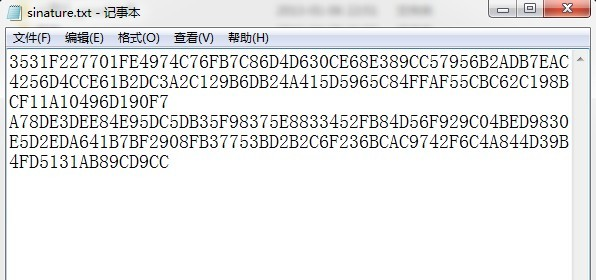
\includegraphics{img/12.jpg}
\caption{验证签名}
\end{figure}

改变data.txt的内容为:

\begin{figure}[H]
\centering
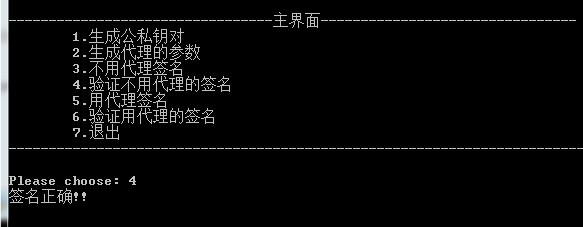
\includegraphics{img/13.jpg}
\caption{原data.txt被修改后}
\end{figure}

然后执行一次验证签名操作结果如下:

\begin{figure}[H]
\centering

\includegraphics{img/14.jpg}
\caption{签名有误}
\end{figure}

对大小为340字节的data.txt进行一组同样的操作

Data.txt

\begin{figure}[H]
\centering
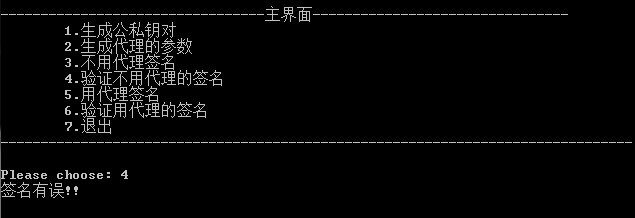
\includegraphics{img/15.jpg}
\caption{data.txt}
\end{figure}

签名

\begin{figure}[H]
\centering
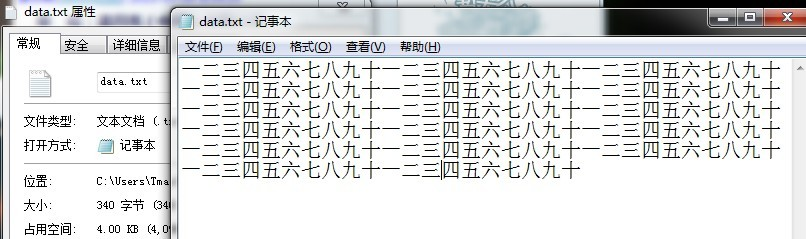
\includegraphics{img/16.jpg}
\caption{签名}
\end{figure}

验证签名

\begin{figure}[H]
\centering
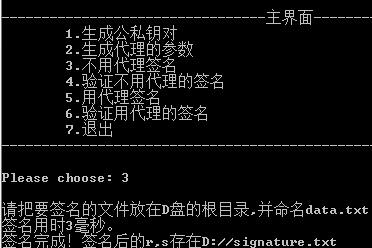
\includegraphics{img/17.jpg}
\caption{验证签名}
\end{figure}

改变data.txt的内容

\begin{figure}[H]
\centering
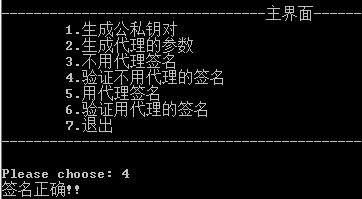
\includegraphics{img/18.jpg}
\caption{data.txt被修改}
\end{figure}

再验证一次签名

\begin{figure}[H]
\centering
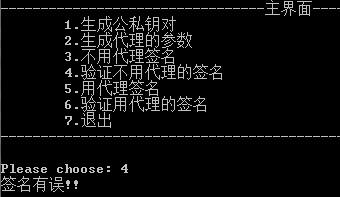
\includegraphics{img/20.jpg}
\caption{原文被改后签名有误}
\end{figure}

\subsubsection{结果分析}

如上面步骤所示,对不同长度data.txt进行签名和对data.txt验证签名得到了与预期相符的结果;而后面原文被窜改,依然对同样的签名进行验证签名,得到的结果是签名有误!与预期结果相符。

\subsection{基于Elgamal算法的代理签名方案的实现}

\subsubsection{测试用例}

测试用例:1、大小为128字节的txt文档。

          2、大小为340字节的txt文档。

\subsubsection{测试过程}

1)  进入系统主界面,选1生成公私钥对,在有了pub.txt和pri.txt数据的情况下,生成代理签名的参数。私密共享给代理签名者的参数d,K,p,g存入proxy\_pri.txt,公布出去的原始签名者的公钥y,代理参数K,p与g存入proxy\_pub.txt中:

\begin{figure}[H]
\centering
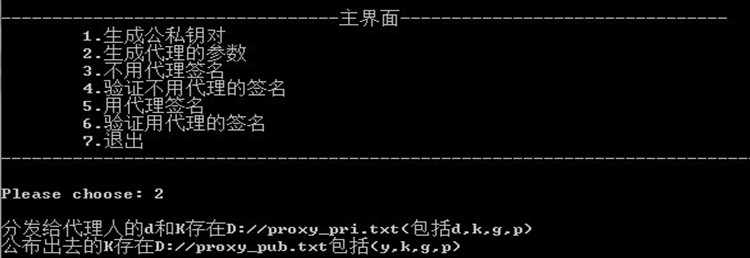
\includegraphics{img/21.jpg}
\caption{proxykeys}
\end{figure}

Proxy\_pri.txt中,由上至下分别为x,K,p,g:

\begin{figure}[H]
\centering
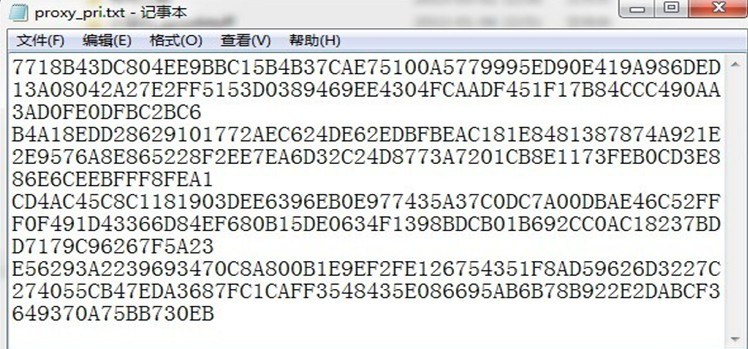
\includegraphics{img/22.jpg}
\caption{proxy\_pri.txt}
\end{figure}

Proxy\_pub.txt中,由上至下分别为原始签名者的公钥y,代理参数K,p与g:

\begin{figure}[H]
\centering
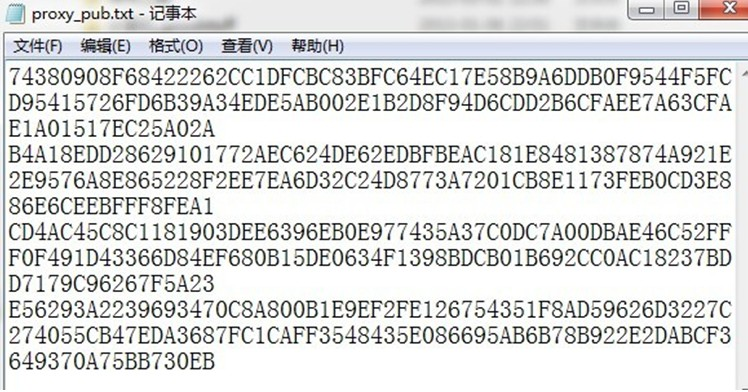
\includegraphics{img/23.jpg}
\caption{proxy\_pub.txt}
\end{figure}

2)  代理签名与验证代理签名

对大小为128字节的data.txt使用代理密钥进行数字签名操作,此步骤包涵对代理参数的检验,即每一次签名前都会检验代理参数是否有效。

\begin{figure}[H]
\centering
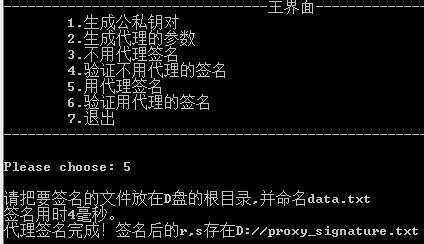
\includegraphics{img/24.jpg}
\caption{proxy-signature}
\end{figure}

签名耗时4毫秒,得到的代理签名(R,s):

\begin{figure}[H]
\centering
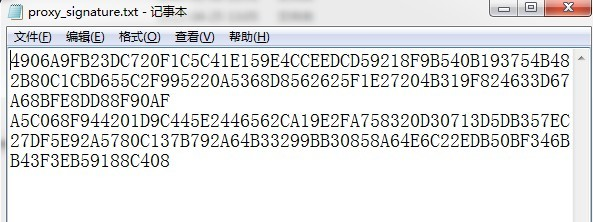
\includegraphics{img/25.jpg}
\caption{proxy-signature.txt}
\end{figure}

验证代理签名,签名正确:

\begin{figure}[H]
\centering
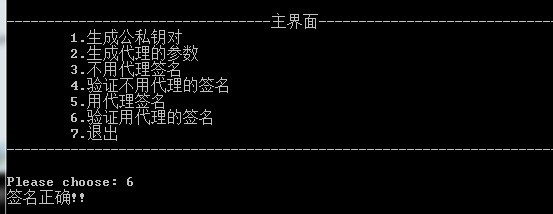
\includegraphics{img/26.jpg}
\caption{签名正确}
\end{figure}

修改data.txt内容为:

\begin{figure}[H]
\centering

\includegraphics{img/28.jpg}
\caption{修改后的data.txt}
\end{figure}

再验证Elgamal代理签名:

\begin{figure}[H]
\centering
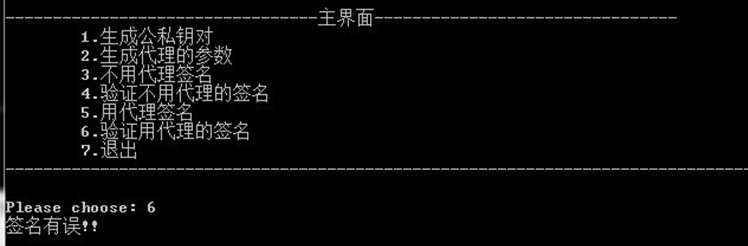
\includegraphics{img/29.jpg}
\caption{原文被改,代理签名有误}
\end{figure}

对大小为340字节的data.txt文档进行一组同上的代理签名与代理签名验证的操作:

data.txt:

\begin{figure}[H]
\centering

\includegraphics{img/30.jpg}
\caption{340字节的data.txt}
\end{figure}

进行代理签名:

\begin{figure}[H]
\centering
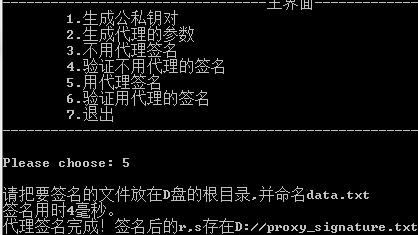
\includegraphics{img/31.jpg}
\caption{代理签名}
\end{figure}

验证代理签名

\begin{figure}[H]
\centering
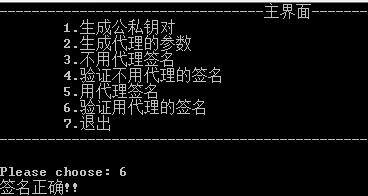
\includegraphics{img/32.jpg}
\caption{验证代理签名,正确!}
\end{figure}

修改data.txt为:

\begin{figure}[H]
\centering

\includegraphics{img/33.jpg}
\caption{修改后的data.txt}
\end{figure}

再验证一次代理签名

\begin{figure}[H]
\centering
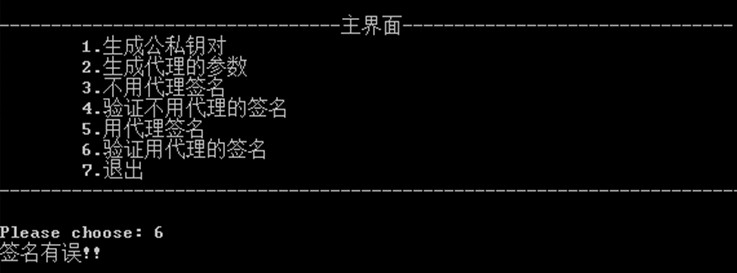
\includegraphics{img/34.jpg}
\caption{原文被改,代理签名验证有误}
\end{figure}

\subsubsection{结果分析}

如上面步骤所示,对不同大小的data.txt进行签名和之后对data\cite{Designated}.txt验证签名都得到了预期的结果,与预期结果相符;而后面原文被窜改,依然对同样的签名进行验证代理签名操作,得到的结果是签名有误!与预期结果相符\cite{计算机密码学及其应用}。
\section{结论}

通过对数字签名及代理签名的理解,以及对Elgamal签名方案的研究,成功使用Microsoft visual C++ 软件运用C语言写出实现Elgamal签名方案及代理签名方案功能的程序,此程序可以对数据进行签名及签名验证和代理签名及代理签名验证。但此程序也有其不足之处,比如没有实现可所有文件格式进行签名的功能,没有把代理及正常签名分开实现,界面不够直观美观,本文实现的代理签名安全性不高,未能达到完美,希望在今后的时间里可以对代理签名的安全性做进一步的加强,并加上一个更具体验价值的用户界面。总的来说,虽不完美,但是实现了Elgamal签名方案和代理签名方案的思想。
%\section{引\hspace{1em}用}
\subsection{Sous section présentant les Références}

\subsubsection{Références bibliographique}

Référence bibliographique simple~\cite{Amendola2017}.

Multiples références bibliographiques en une seule commande~\cite{Petkov2005,Raman2009,Colinet2004}.


\subsubsection{Références aux équations, figures, et tables}

Voir l'équation~\eqref{eq:equation}. Voir \autoref{fig:label} et la figure~\ref{fig:label}.

Voir le tableau~\ref{table:tableaucomplexe} page~\pageref{table:tableaucomplexe}.


\appendix\titlecontents{section}[0pt]{\vspace{.5\baselineskip}\bfseries}
{附录\thecontentslabel\quad}{}
{\hspace{.5em}\titlerule*[10pt]{$\cdot$}\contentspage}
\titleformat{\section}{\centering\LARGE\bfseries}{附录%
\,\thesection}{1em}{}
%\chapter{外文资料原文}
\label{cha:engorg}

\title{The title of the English paper}

\textbf{Abstract:} As one of the most widely used techniques in operations
research, \emph{ mathematical programming} is defined as a means of maximizing a
quantity known as \emph{bjective function}, subject to a set of constraints
represented by equations and inequalities. Some known subtopics of mathematical
programming are linear programming, nonlinear programming, multiobjective
programming, goal programming, dynamic programming, and multilevel
programming$^{[1]}$.

It is impossible to cover in a single chapter every concept of mathematical
programming. This chapter introduces only the basic concepts and techniques of
mathematical programming such that readers gain an understanding of them
throughout the book$^{[2,3]}$.


\section{Single-Objective Programming}
The general form of single-objective programming (SOP) is written
as follows,
\begin{equation*} % 如果附录中的公式不想让它出现在公式索引中,那就请
                             % 用 equation*
\left\{\begin{array}{l}
\max \,\,f(x)\\[0.1 cm]
\mbox{subject to:} \\ [0.1 cm]
\qquad g_j(x)\le 0,\quad j=1,2,\cdots,p
\end{array}\right.
\end{equation*}
which maximizes a real-valued function $f$ of
$x=(x_1,x_2,\cdots,x_n)$ subject to a set of constraints.

\newcommand\Real{\mathbf{R}}
\newtheorem{mpdef}{Definition}[chapter]
\begin{mpdef}
In SOP, we call $x$ a decision vector, and
$x_1,x_2,\cdots,x_n$ decision variables. The function
$f$ is called the objective function. The set
\begin{equation*}
S=\left\{x\in\Real^n\bigm|g_j(x)\le 0,\,j=1,2,\cdots,p\right\}
\end{equation*}
is called the feasible set. An element $x$ in $S$ is called a
feasible solution.
\end{mpdef}

\newtheorem{mpdefop}[mpdef]{Definition}
\begin{mpdefop}
A feasible solution $x^*$ is called the optimal
solution of SOP if and only if
\begin{equation}
f(x^*)\ge f(x)
\end{equation}
for any feasible solution $x$.
\end{mpdefop}

One of the outstanding contributions to mathematical programming was known as
the Kuhn-Tucker conditions\ref{eq:ktc}. In order to introduce them, let us give
some definitions. An inequality constraint $g_j(x)\le 0$ is said to be active at
a point $x^*$ if $g_j(x^*)=0$. A point $x^*$ satisfying $g_j(x^*)\le 0$ is said
to be regular if the gradient vectors $\nabla g_j(x)$ of all active constraints
are linearly independent.

Let $x^*$ be a regular point of the constraints of SOP and assume that all the
functions $f(x)$ and $g_j(x),j=1,2,\cdots,p$ are differentiable. If $x^*$ is a
local optimal solution, then there exist Lagrange multipliers
$\lambda_j,j=1,2,\cdots,p$ such that the following Kuhn-Tucker conditions hold,
\begin{equation}
\label{eq:ktc}
\left\{\begin{array}{l}
    \nabla f(x^*)-\sum\limits_{j=1}^p\lambda_j\nabla g_j(x^*)=0\\[0.3cm]
    \lambda_jg_j(x^*)=0,\quad j=1,2,\cdots,p\\[0.2cm]
    \lambda_j\ge 0,\quad j=1,2,\cdots,p.
\end{array}\right.
\end{equation}
If all the functions $f(x)$ and $g_j(x),j=1,2,\cdots,p$ are convex and
differentiable, and the point $x^*$ satisfies the Kuhn-Tucker conditions
(\ref{eq:ktc}), then it has been proved that the point $x^*$ is a global optimal
solution of SOP.

\subsection{Linear Programming}
\label{sec:lp}

If the functions $f(x),g_j(x),j=1,2,\cdots,p$ are all linear, then SOP is called
a {\em linear programming}.

The feasible set of linear is always convex. A point $x$ is called an extreme
point of convex set $S$ if $x\in S$ and $x$ cannot be expressed as a convex
combination of two points in $S$. It has been shown that the optimal solution to
linear programming corresponds to an extreme point of its feasible set provided
that the feasible set $S$ is bounded. This fact is the basis of the {\em simplex
  algorithm} which was developed by Dantzig as a very efficient method for
solving linear programming.
\begin{table}[ht]
\centering
  \centering
  \caption*{Table~1\hskip1em This is an example for manually numbered table, which
    would not appear in the list of tables}
  \label{tab:badtabular2}
  \begin{tabular}[c]{|m{1.5cm}|c|c|c|c|c|c|}\hline
    \multicolumn{2}{|c|}{Network Topology} & \# of nodes &
    \multicolumn{3}{c|}{\# of clients} & Server \\\hline
    GT-ITM & Waxman Transit-Stub & 600 &
    \multirow{2}{2em}{2\%}&
    \multirow{2}{2em}{10\%}&
    \multirow{2}{2em}{50\%}&
    \multirow{2}{1.2in}{Max. Connectivity}\\\cline{1-3}
    \multicolumn{2}{|c|}{Inet-2.1} & 6000 & & & &\\\hline
    \multirow{2}{1.5cm}{Xue} & Rui  & Ni &\multicolumn{4}{c|}{\multirow{2}*{\thuthesis}}\\\cline{2-3}
    & \multicolumn{2}{c|}{ABCDEF} &\multicolumn{4}{c|}{} \\\hline
\end{tabular}
\end{table}

Roughly speaking, the simplex algorithm examines only the extreme points of the
feasible set, rather than all feasible points. At first, the simplex algorithm
selects an extreme point as the initial point. The successive extreme point is
selected so as to improve the objective function value. The procedure is
repeated until no improvement in objective function value can be made. The last
extreme point is the optimal solution.

\subsection{Nonlinear Programming}

If at least one of the functions $f(x),g_j(x),j=1,2,\cdots,p$ is nonlinear, then
SOP is called a {\em nonlinear programming}.

A large number of classical optimization methods have been developed to treat
special-structural nonlinear programming based on the mathematical theory
concerned with analyzing the structure of problems.
\begin{figure}[h]
  \centering
  
\includegraphics{thu-lib-logo.pdf}
  \caption*{Figure~1\quad This is an example for manually numbered figure,
    which would not appear in the list of figures}
  \label{tab:badfigure2}
\end{figure}

Now we consider a nonlinear programming which is confronted solely with
maximizing a real-valued function with domain $\Real^n$.  Whether derivatives are
available or not, the usual strategy is first to select a point in $\Real^n$ which
is thought to be the most likely place where the maximum exists. If there is no
information available on which to base such a selection, a point is chosen at
random. From this first point an attempt is made to construct a sequence of
points, each of which yields an improved objective function value over its
predecessor. The next point to be added to the sequence is chosen by analyzing
the behavior of the function at the previous points. This construction continues
until some termination criterion is met. Methods based upon this strategy are
called {\em ascent methods}, which can be classified as {\em direct methods},
{\em gradient methods}, and {\em Hessian methods} according to the information
about the behavior of objective function $f$. Direct methods require only that
the function can be evaluated at each point. Gradient methods require the
evaluation of first derivatives of $f$. Hessian methods require the evaluation
of second derivatives. In fact, there is no superior method for all
problems. The efficiency of a method is very much dependent upon the objective
function.

\subsection{Integer Programming}

{\em Integer programming} is a special mathematical programming in which all of
the variables are assumed to be only integer values. When there are not only
integer variables but also conventional continuous variables, we call it {\em
  mixed integer programming}. If all the variables are assumed either 0 or 1,
then the problem is termed a {\em zero-one programming}. Although integer
programming can be solved by an {\em exhaustive enumeration} theoretically, it
is impractical to solve realistically sized integer programming problems. The
most successful algorithm so far found to solve integer programming is called
the {\em branch-and-bound enumeration} developed by Balas (1965) and Dakin
(1965). The other technique to integer programming is the {\em cutting plane
  method} developed by Gomory (1959).

\hfill\textit{Uncertain Programming\/}\quad(\textsl{BaoDing Liu, 2006.2})

\section*{References}
\noindent{\itshape NOTE: These references are only for demonstration. They are
  not real citations in the original text.}

\begin{translationbib}
\item Donald E. Knuth. The \TeX book. Addison-Wesley, 1984. ISBN: 0-201-13448-9
\item Paul W. Abrahams, Karl Berry and Kathryn A. Hargreaves. \TeX\ for the
  Impatient. Addison-Wesley, 1990. ISBN: 0-201-51375-7
\item David Salomon. The advanced \TeX book.  New York : Springer, 1995. ISBN:0-387-94556-3
\end{translationbib}

\chapter{外文资料的调研阅读报告或书面翻译}

\title{英文资料的中文标题}

{\heiti 摘要:} 本章为外文资料翻译内容。如果有摘要可以直接写上来,这部分好像没有
明确的规定。

\section{单目标规划}
北冥有鱼,其名为鲲。鲲之大,不知其几千里也。化而为鸟,其名为鹏。鹏之背,不知其几
千里也。怒而飞,其翼若垂天之云。是鸟也,海运则将徙于南冥。南冥者,天池也。
\begin{equation}\tag*{(123)}
 p(y|\mathbf{x}) = \frac{p(\mathbf{x},y)}{p(\mathbf{x})}=
\frac{p(\mathbf{x}|y)p(y)}{p(\mathbf{x})}
\end{equation}

吾生也有涯,而知也无涯。以有涯随无涯,殆已!已而为知者,殆而已矣!为善无近名,为
恶无近刑,缘督以为经,可以保身,可以全生,可以养亲,可以尽年。

\subsection{线性规划}
庖丁为文惠君解牛,手之所触,肩之所倚,足之所履,膝之所倚,砉然响然,奏刀騞然,莫
不中音,合于桑林之舞,乃中经首之会。
\begin{table}[ht]
\centering
  \centering
  \caption*{表~1\hskip1em 这是手动编号但不出现在索引中的一个表格例子}
  \label{tab:badtabular3}
  \begin{tabular}[c]{|m{1.5cm}|c|c|c|c|c|c|}\hline
    \multicolumn{2}{|c|}{Network Topology} & \# of nodes &
    \multicolumn{3}{c|}{\# of clients} & Server \\\hline
    GT-ITM & Waxman Transit-Stub & 600 &
    \multirow{2}{2em}{2\%}&
    \multirow{2}{2em}{10\%}&
    \multirow{2}{2em}{50\%}&
    \multirow{2}{1.2in}{Max. Connectivity}\\\cline{1-3}
    \multicolumn{2}{|c|}{Inet-2.1} & 6000 & & & &\\\hline
    \multirow{2}{1.5cm}{Xue} & Rui  & Ni &\multicolumn{4}{c|}{\multirow{2}*{\thuthesis}}\\\cline{2-3}
    & \multicolumn{2}{c|}{ABCDEF} &\multicolumn{4}{c|}{} \\\hline
\end{tabular}
\end{table}

文惠君曰:“嘻,善哉!技盖至此乎?”庖丁释刀对曰:“臣之所好者道也,进乎技矣。始臣之
解牛之时,所见无非全牛者;三年之后,未尝见全牛也;方今之时,臣以神遇而不以目视,
官知止而神欲行。依乎天理,批大郤,导大窾,因其固然。技经肯綮之未尝,而况大坬乎!
良庖岁更刀,割也;族庖月更刀,折也;今臣之刀十九年矣,所解数千牛矣,而刀刃若新发
于硎。彼节者有间而刀刃者无厚,以无厚入有间,恢恢乎其于游刃必有余地矣。是以十九年
而刀刃若新发于硎。虽然,每至于族,吾见其难为,怵然为戒,视为止,行为迟,动刀甚微,
謋然已解,如土委地。提刀而立,为之而四顾,为之踌躇满志,善刀而藏之。”

文惠君曰:“善哉!吾闻庖丁之言,得养生焉。”


\subsection{非线性规划}
孔子与柳下季为友,柳下季之弟名曰盗跖。盗跖从卒九千人,横行天下,侵暴诸侯。穴室枢
户,驱人牛马,取人妇女。贪得忘亲,不顾父母兄弟,不祭先祖。所过之邑,大国守城,小
国入保,万民苦之。孔子谓柳下季曰:“夫为人父者,必能诏其子;为人兄者,必能教其弟。
若父不能诏其子,兄不能教其弟,则无贵父子兄弟之亲矣。今先生,世之才士也,弟为盗
跖,为天下害,而弗能教也,丘窃为先生羞之。丘请为先生往说之。”
\begin{figure}[h]
  \centering
  
\includegraphics{thu-whole-logo.pdf}
  \caption*{图~1\hskip1em 这是手动编号但不出现索引中的图片的例子}
  \label{tab:badfigure3}
\end{figure}

柳下季曰:“先生言为人父者必能诏其子,为人兄者必能教其弟,若子不听父之诏,弟不受
兄之教,虽今先生之辩,将奈之何哉?且跖之为人也,心如涌泉,意如飘风,强足以距敌,
辩足以饰非。顺其心则喜,逆其心则怒,易辱人以言。先生必无往。”

孔子不听,颜回为驭,子贡为右,往见盗跖。

\subsection{整数规划}
盗跖乃方休卒徒大山之阳,脍人肝而餔之。孔子下车而前,见谒者曰:“鲁人孔丘,闻将军
高义,敬再拜谒者。”谒者入通。盗跖闻之大怒,目如明星,发上指冠,曰:“此夫鲁国之
巧伪人孔丘非邪?为我告之:尔作言造语,妄称文、武,冠枝木之冠,带死牛之胁,多辞缪
说,不耕而食,不织而衣,摇唇鼓舌,擅生是非,以迷天下之主,使天下学士不反其本,妄
作孝弟,而侥幸于封侯富贵者也。子之罪大极重,疾走归!不然,我将以子肝益昼餔之膳。”


\chapter{其它附录}
前面两个附录主要是给本科生做例子。其它附录的内容可以放到这里,当然如果你愿意,可
以把这部分也放到独立的文件中,然后将其 \cs{input} 到主文件中。

\section*{致谢}\addcontentsline{toc}{section}{致谢}
% ************************** Thesis Acknowledgements **************************

\begin{acknowledgements}      

For what has been an incredibly rewarding and wonderfully challenging 45 months I have several people to thank, several times over. David, for being a superb supervisor, whose unstinting zen and benevolent wisdom are a template for academic mentorship. Richard and Will, who both played the role of unofficial supervisors and always left their doors ajar. Sharon, whose gravitational pull kept me (and everyone else) in orbit. Dan, Mick and John for providing valuable advice along the way. Steve and Bill who as panel members took a much appreciated interest in my progression. Cam who provided valuable insights into my original project proposal. Various other fantastic UNSW folk that have contributed to the fun, including in no particular order: Sam, Sylvia, Eve, Mitch, Nick, Evan, Jo, Chris, Ben, Anna, Chantel, Francis, David and the Ecostats crew, Angela, Haba, Rhiannnon and the rest of the Big Ecology lab. The brilliant academics of the UCT Botany Dept, and in particular Jeremy and Tony who as honours supervisors made me think differently, in a really good way. My patient parents who have supported me unconditionally in my every pursuit. My generous brother who amongst many other things has done his best to keep me in fashion. My wonderful wife Shan, a mention in the acknowledgements of my thesis almost makes a mockery of your contribution; you rock like Kilimanjaro. Finally, I thank my amazing little Ash Mae, who makes me stop and smell the roses (and the nappies).


\end{acknowledgements}


\end{document}